% !TEX root = diss.tex

\chapter{Chapter~\protect\ref{ch:arrhenius} Additional Data}\label{ap:arrhenius}

\begin{figure}[H]
  \centering
  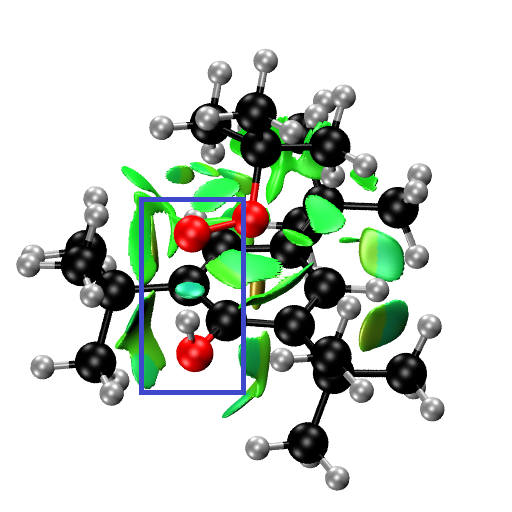
\includegraphics[width=0.9\textwidth]{figures/nciplot.png}
  \caption[NCIplot of complex 5.]{NCIplot\cite{Johnson2010,ContrerasGarcia2011} of complex 5. The blue spheroid (highlighted in the blue box) between the $t$-butylperoxyl oxygen centred radical and the 2,4,6-tri-$t$-butylphenol hydroxyl indicates a hydrogen bonding interaction. The additional green surfaces represent stereo-electronic and weak dispersion interactions.}
  \label{fig:nciplot}
\end{figure}

\begin{figure}[H]
  \centering
  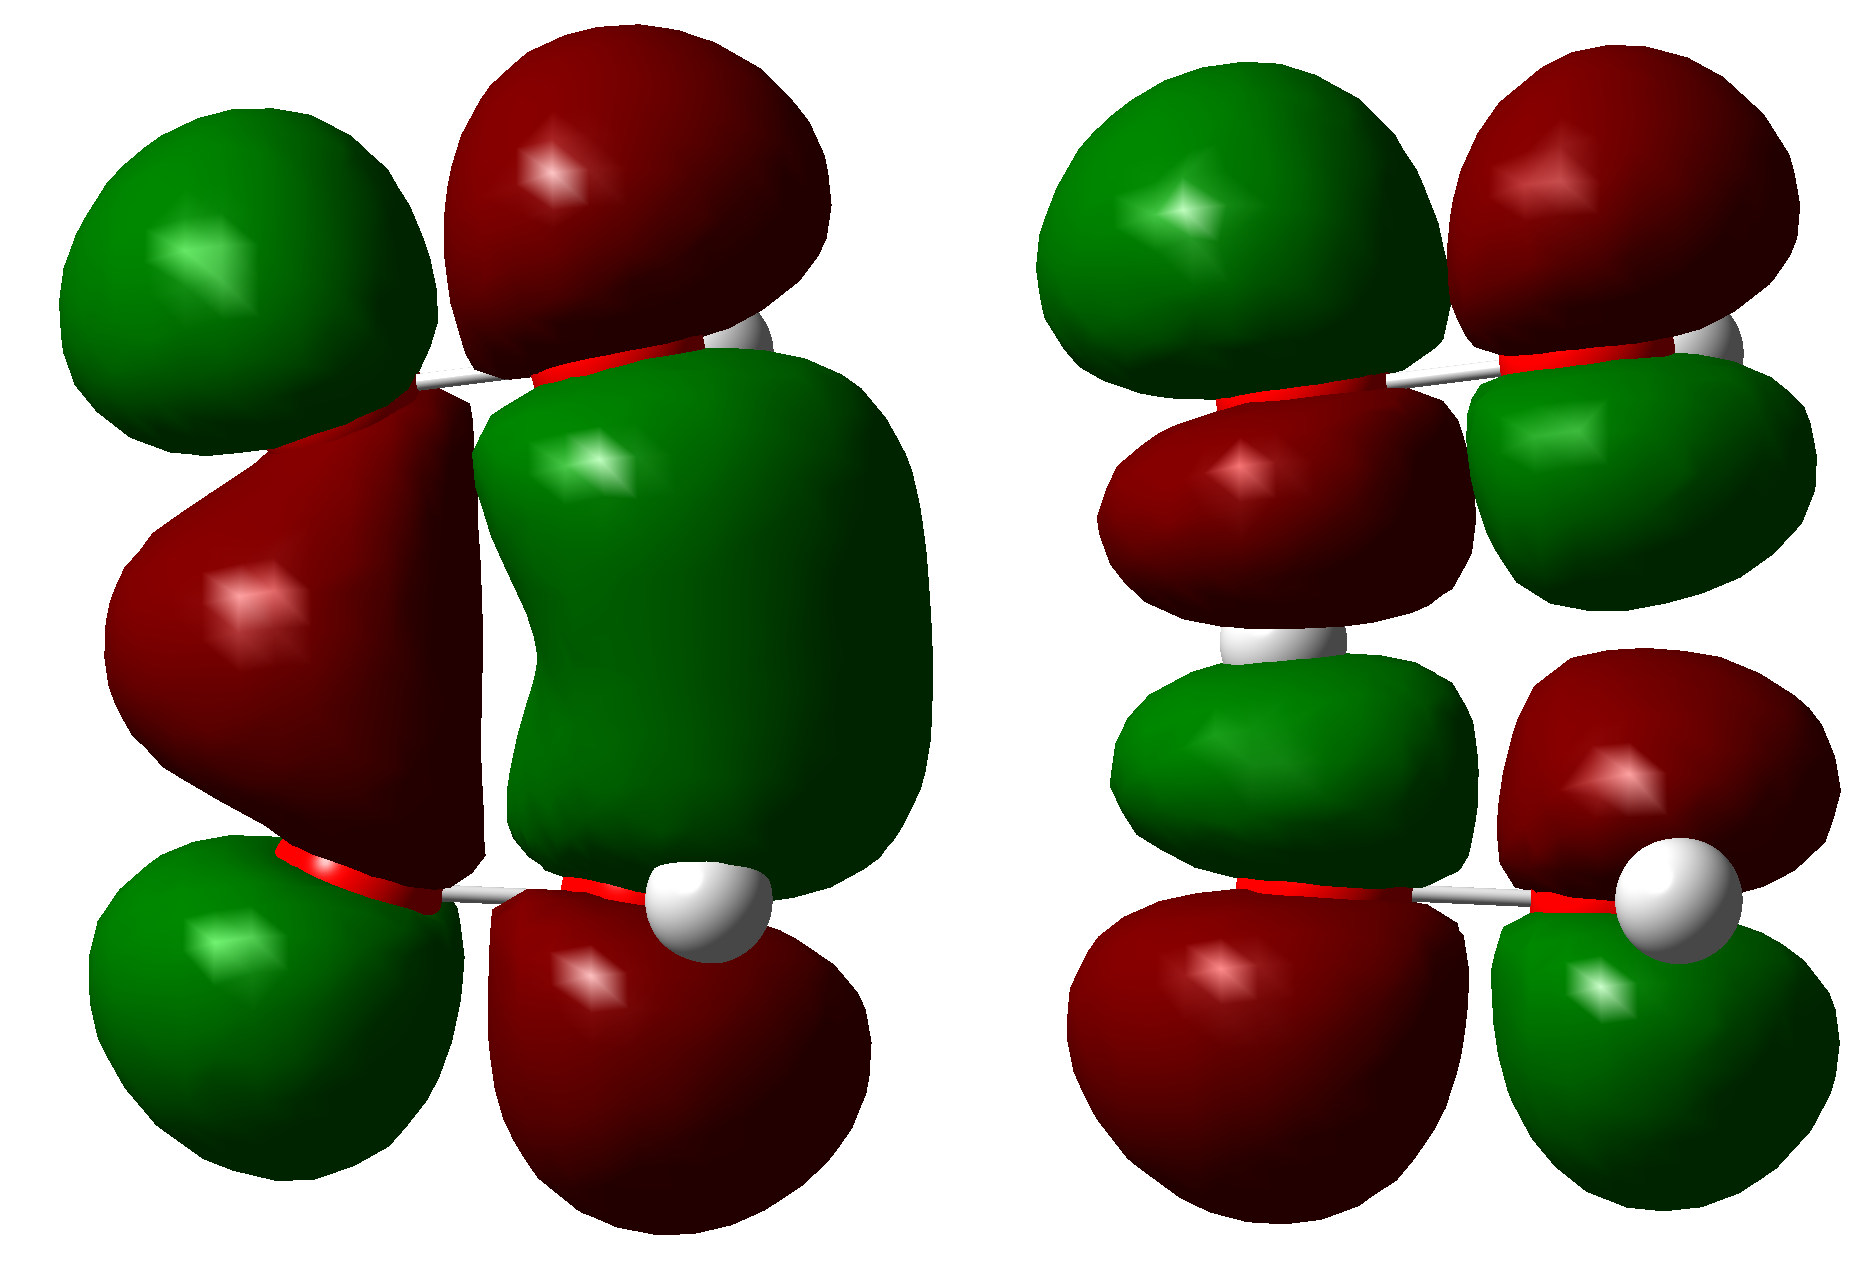
\includegraphics[width=\textwidth]{figures/hoohooh_TS.png}
  \caption[Molecular orbitals of hydrogen peroxide-peroxyl self-exchange reaction TS complex, demonstrating a PCET mechanism.]{Molecular orbitals of hydrogen peroxide-peroxyl self-exchange reaction TS complex, demonstrating a PCET mechanism. Left is the HOMO-1 and right is the SOMO.\@ Together they demonstrate a lone pair-lone pair net half bonding interactions, consistent with PCET.}
  \label{fig:hooh-ooh}
\end{figure}

\chapter{Chapter~\protect\ref{ch:bde} Additional Data}\label{ap:bde}

\begin{figure}[H]
\hspace*{-1.8cm}
\begin{minipage}{8cm}
  \centering
  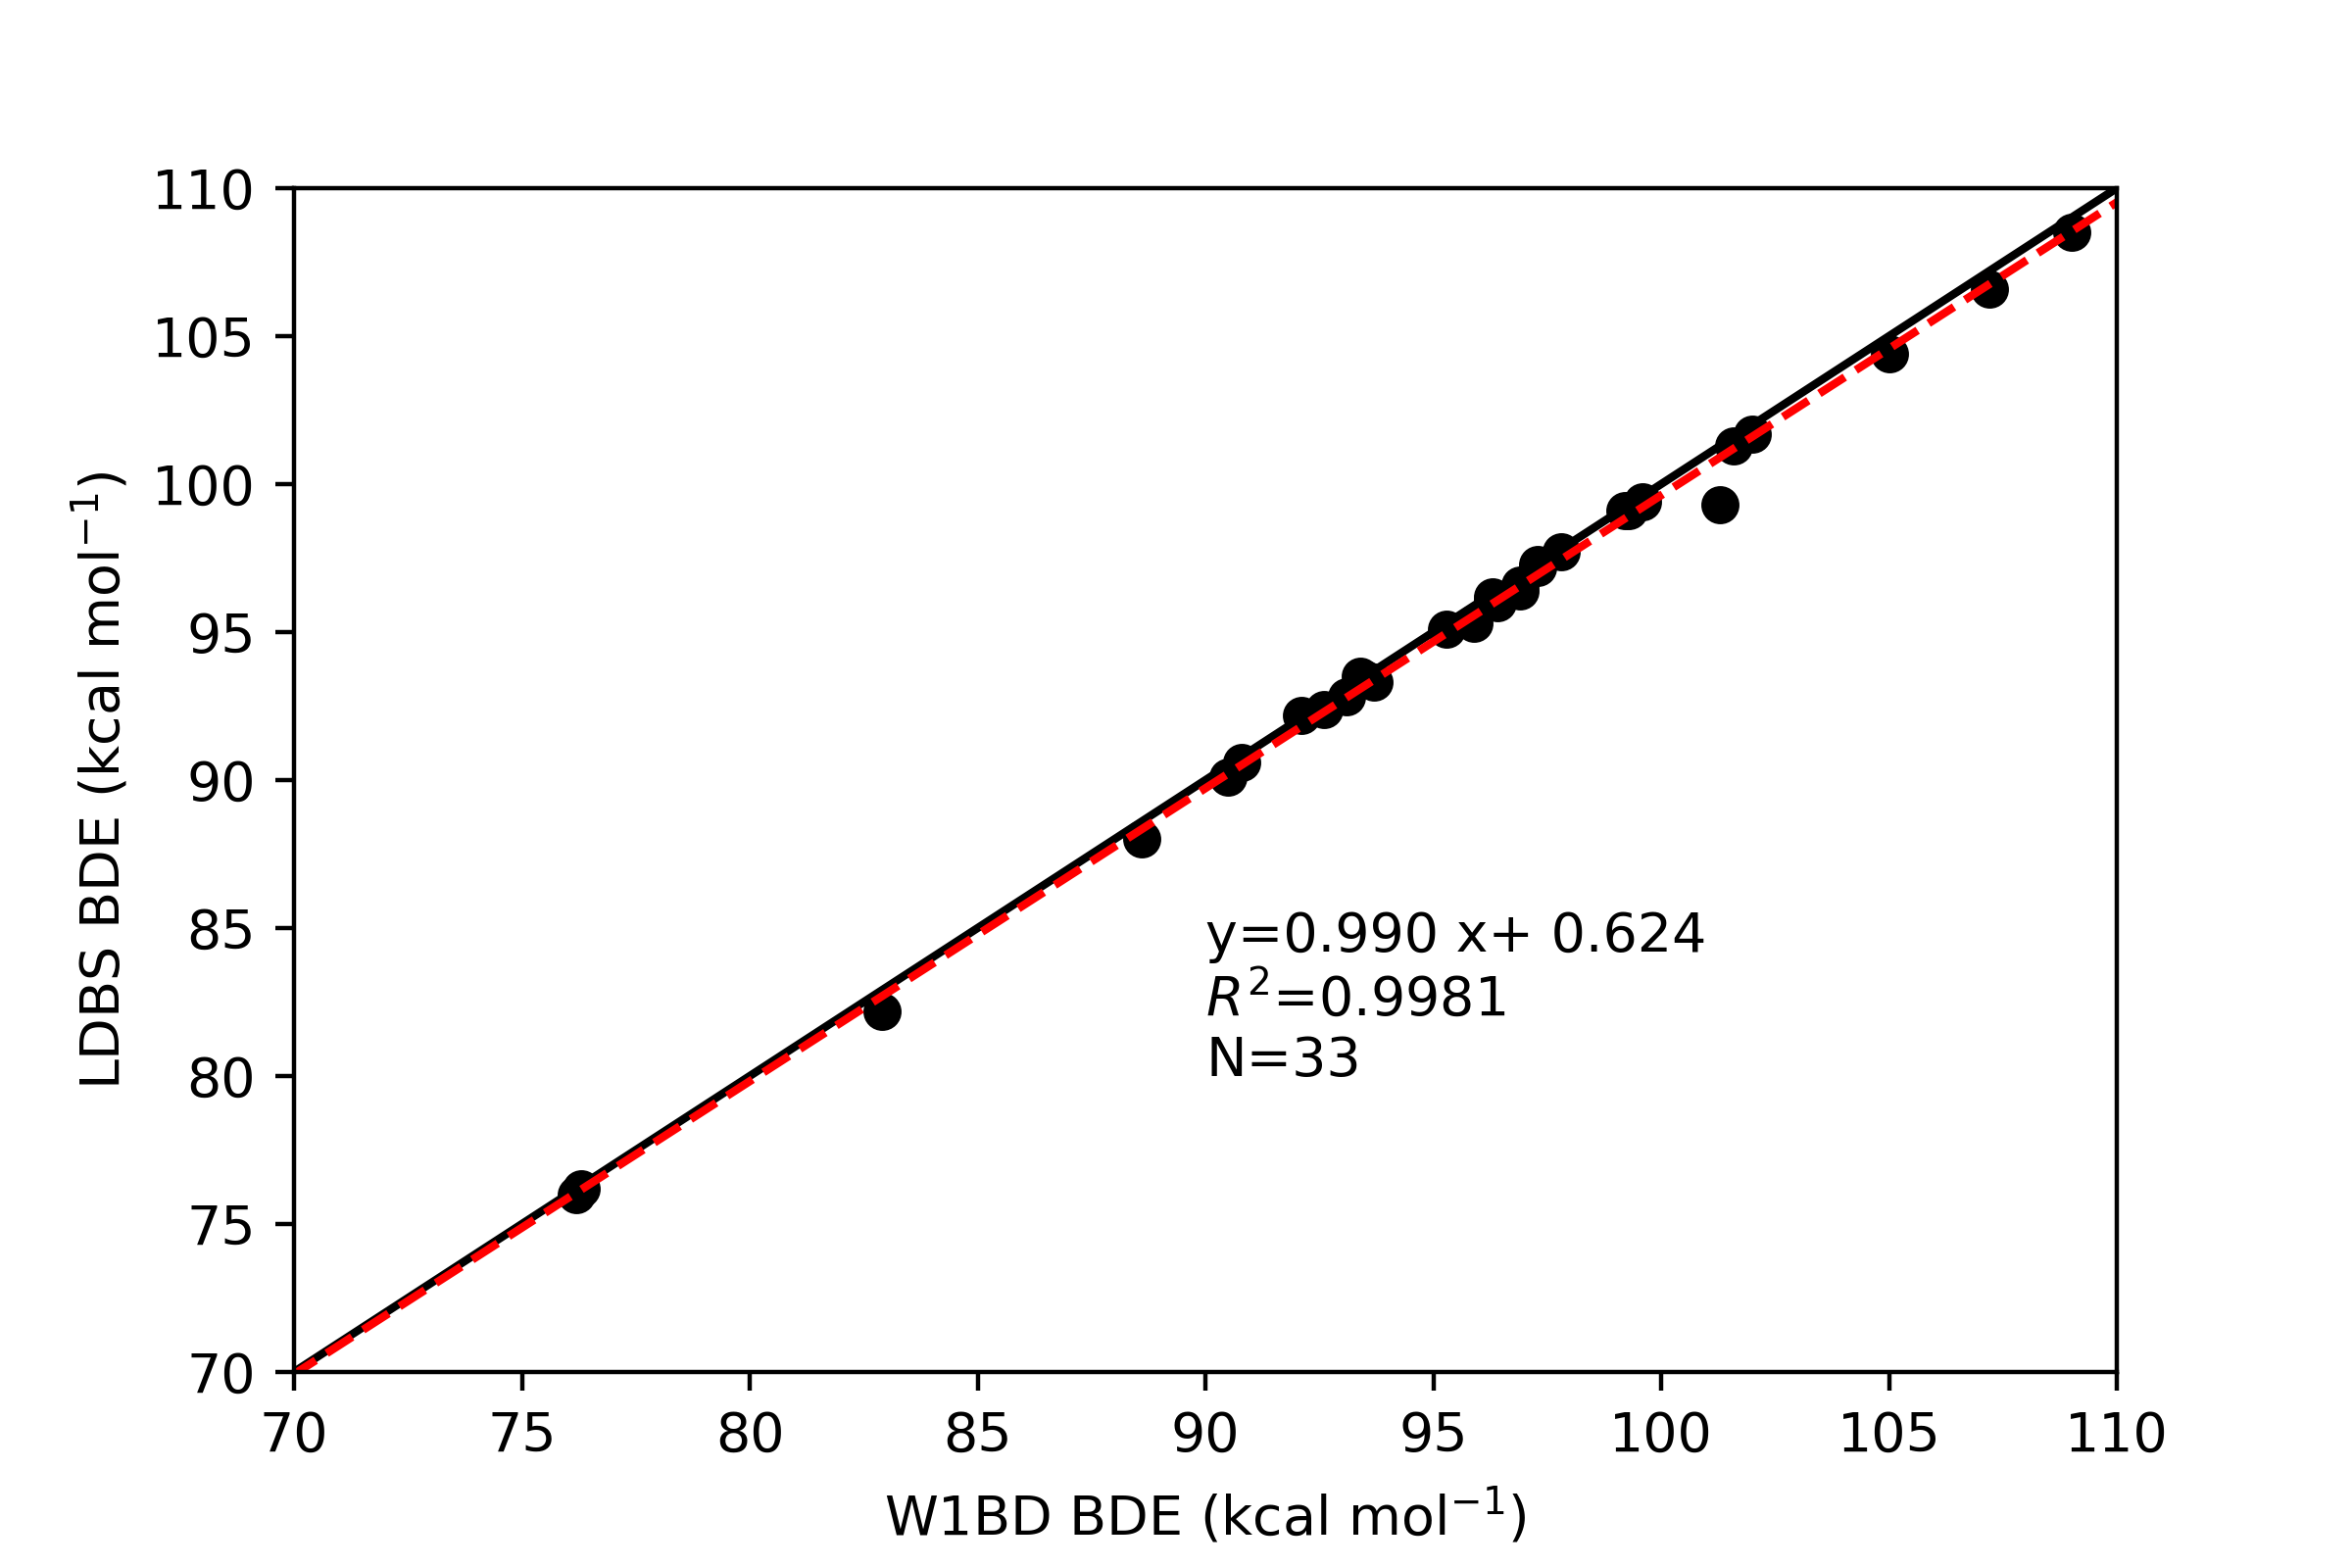
\includegraphics[width=\textwidth]{figures/w1bd-ldbs}
\end{minipage}%
\begin{minipage}{8cm}
  \centering
  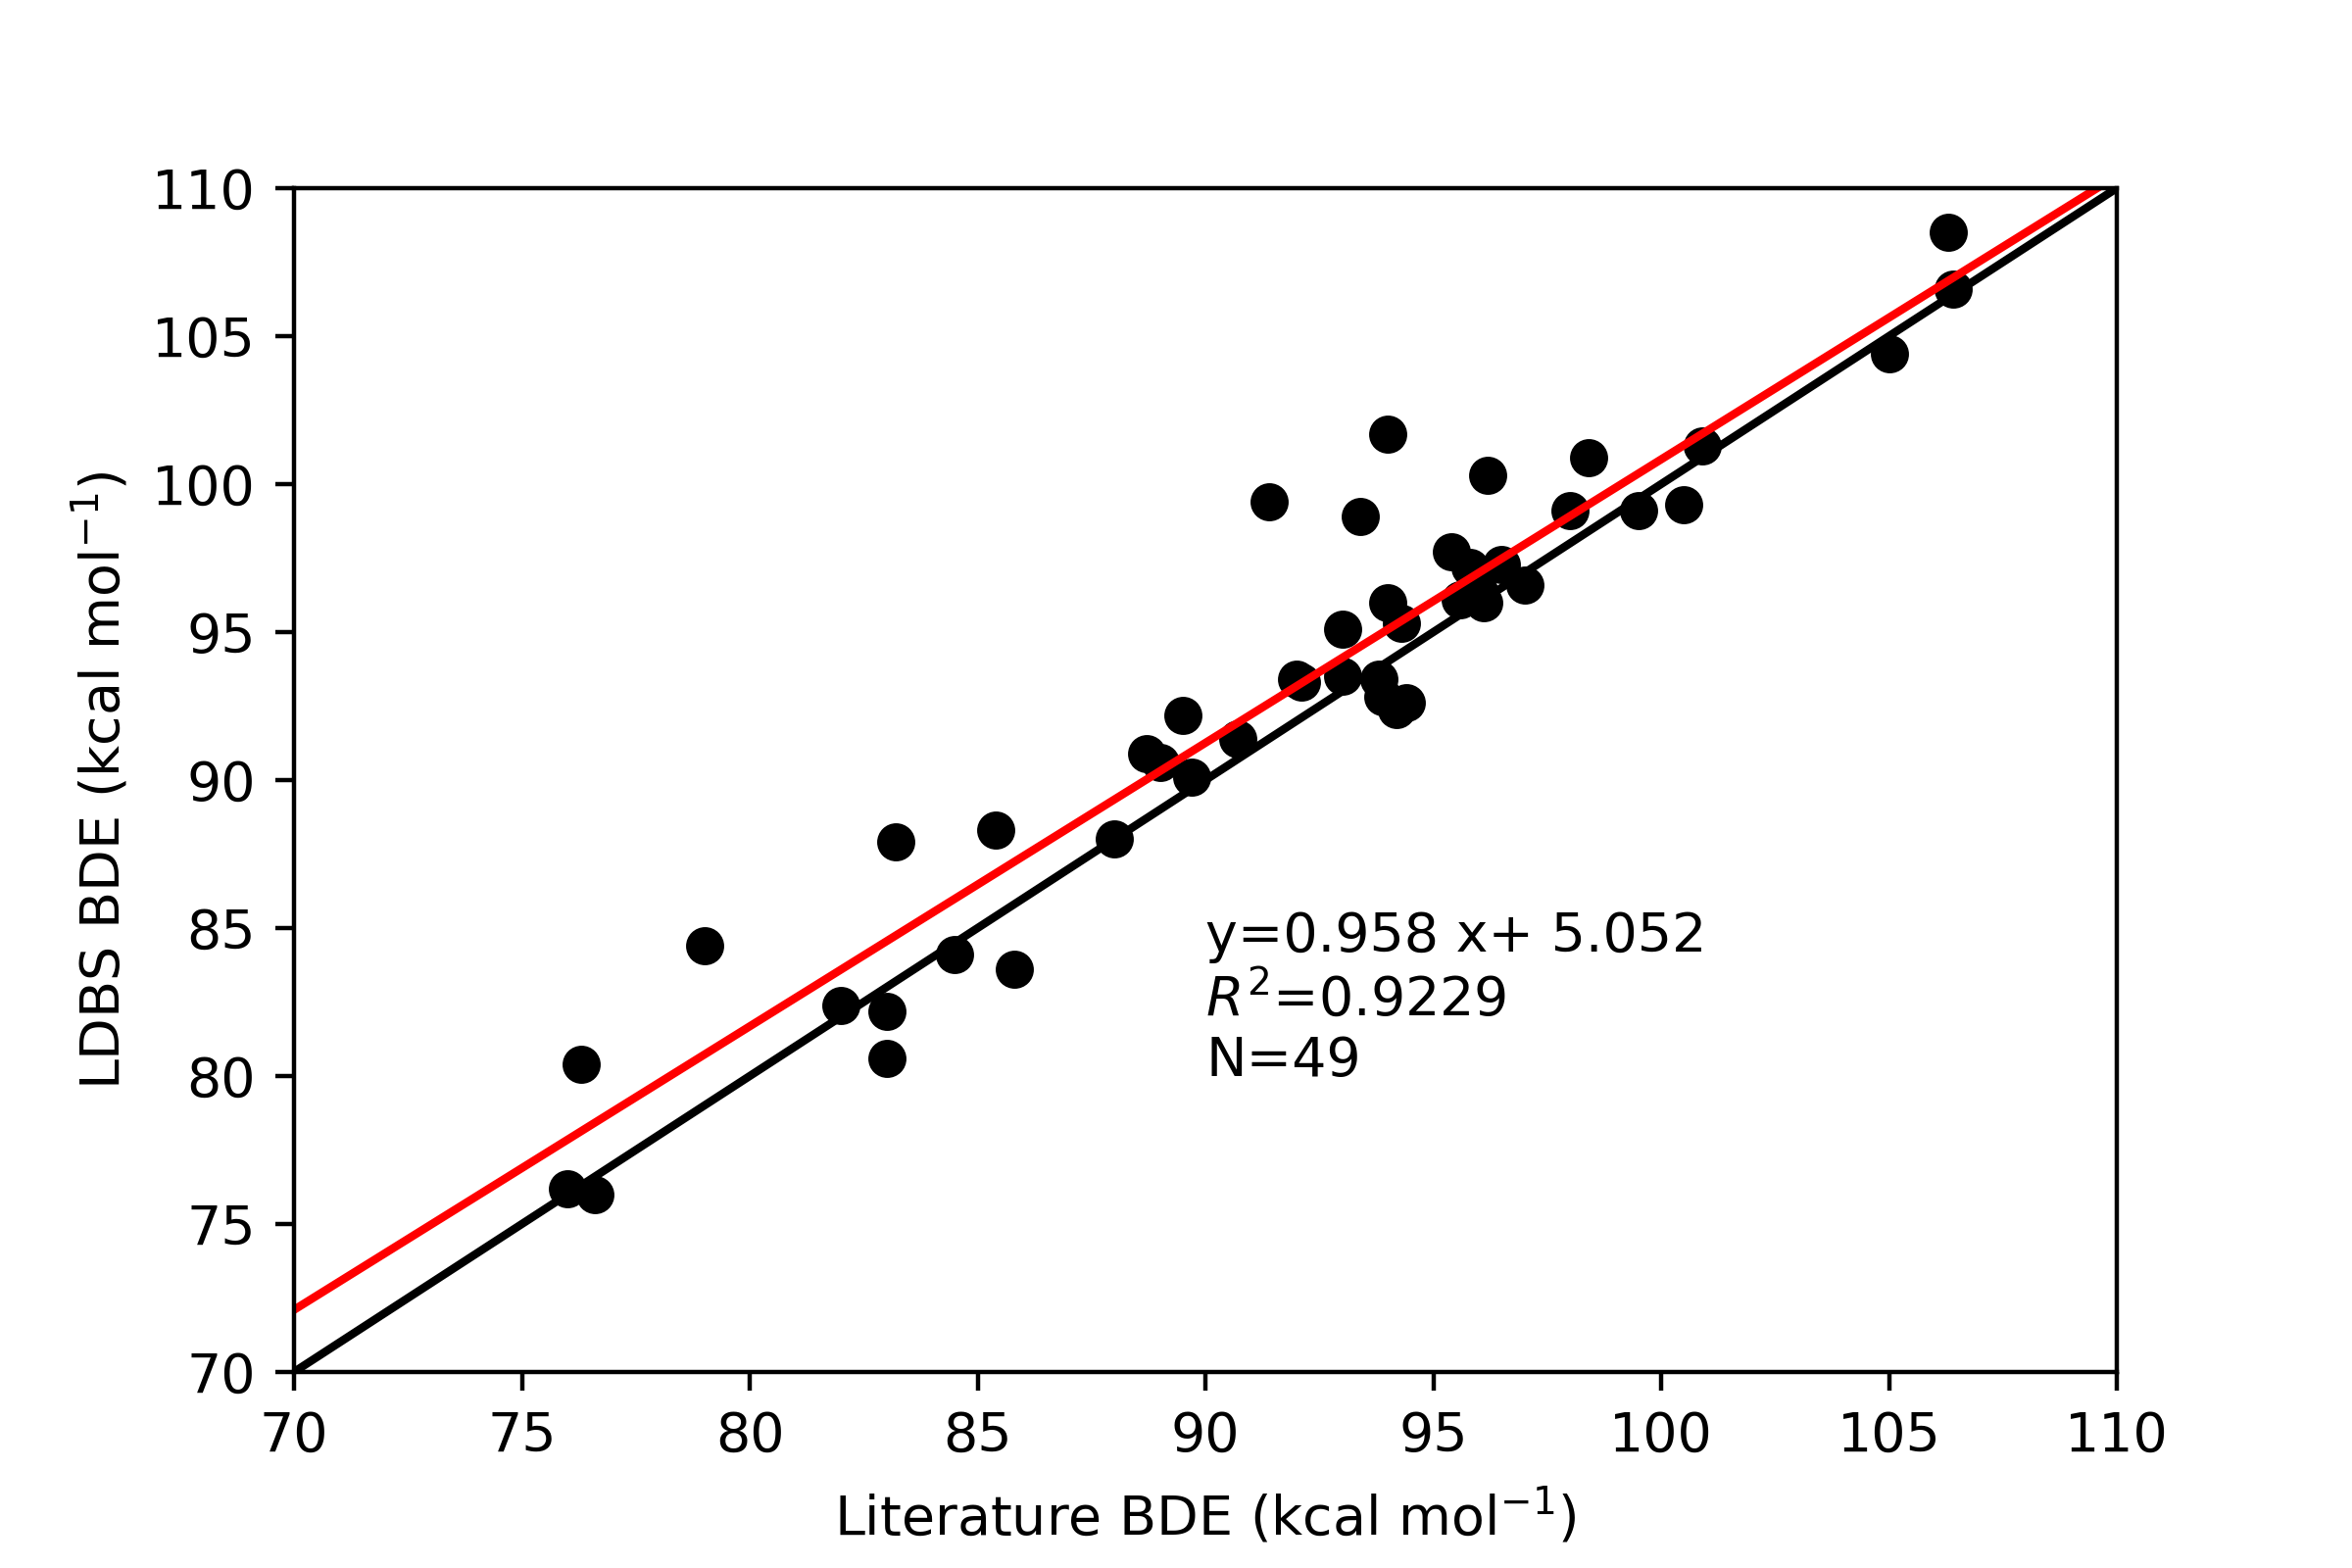
\includegraphics[width=\textwidth]{figures/lit-ldbs}
\end{minipage}

\hspace*{-1.8cm}
\begin{minipage}{8cm}
  \centering
  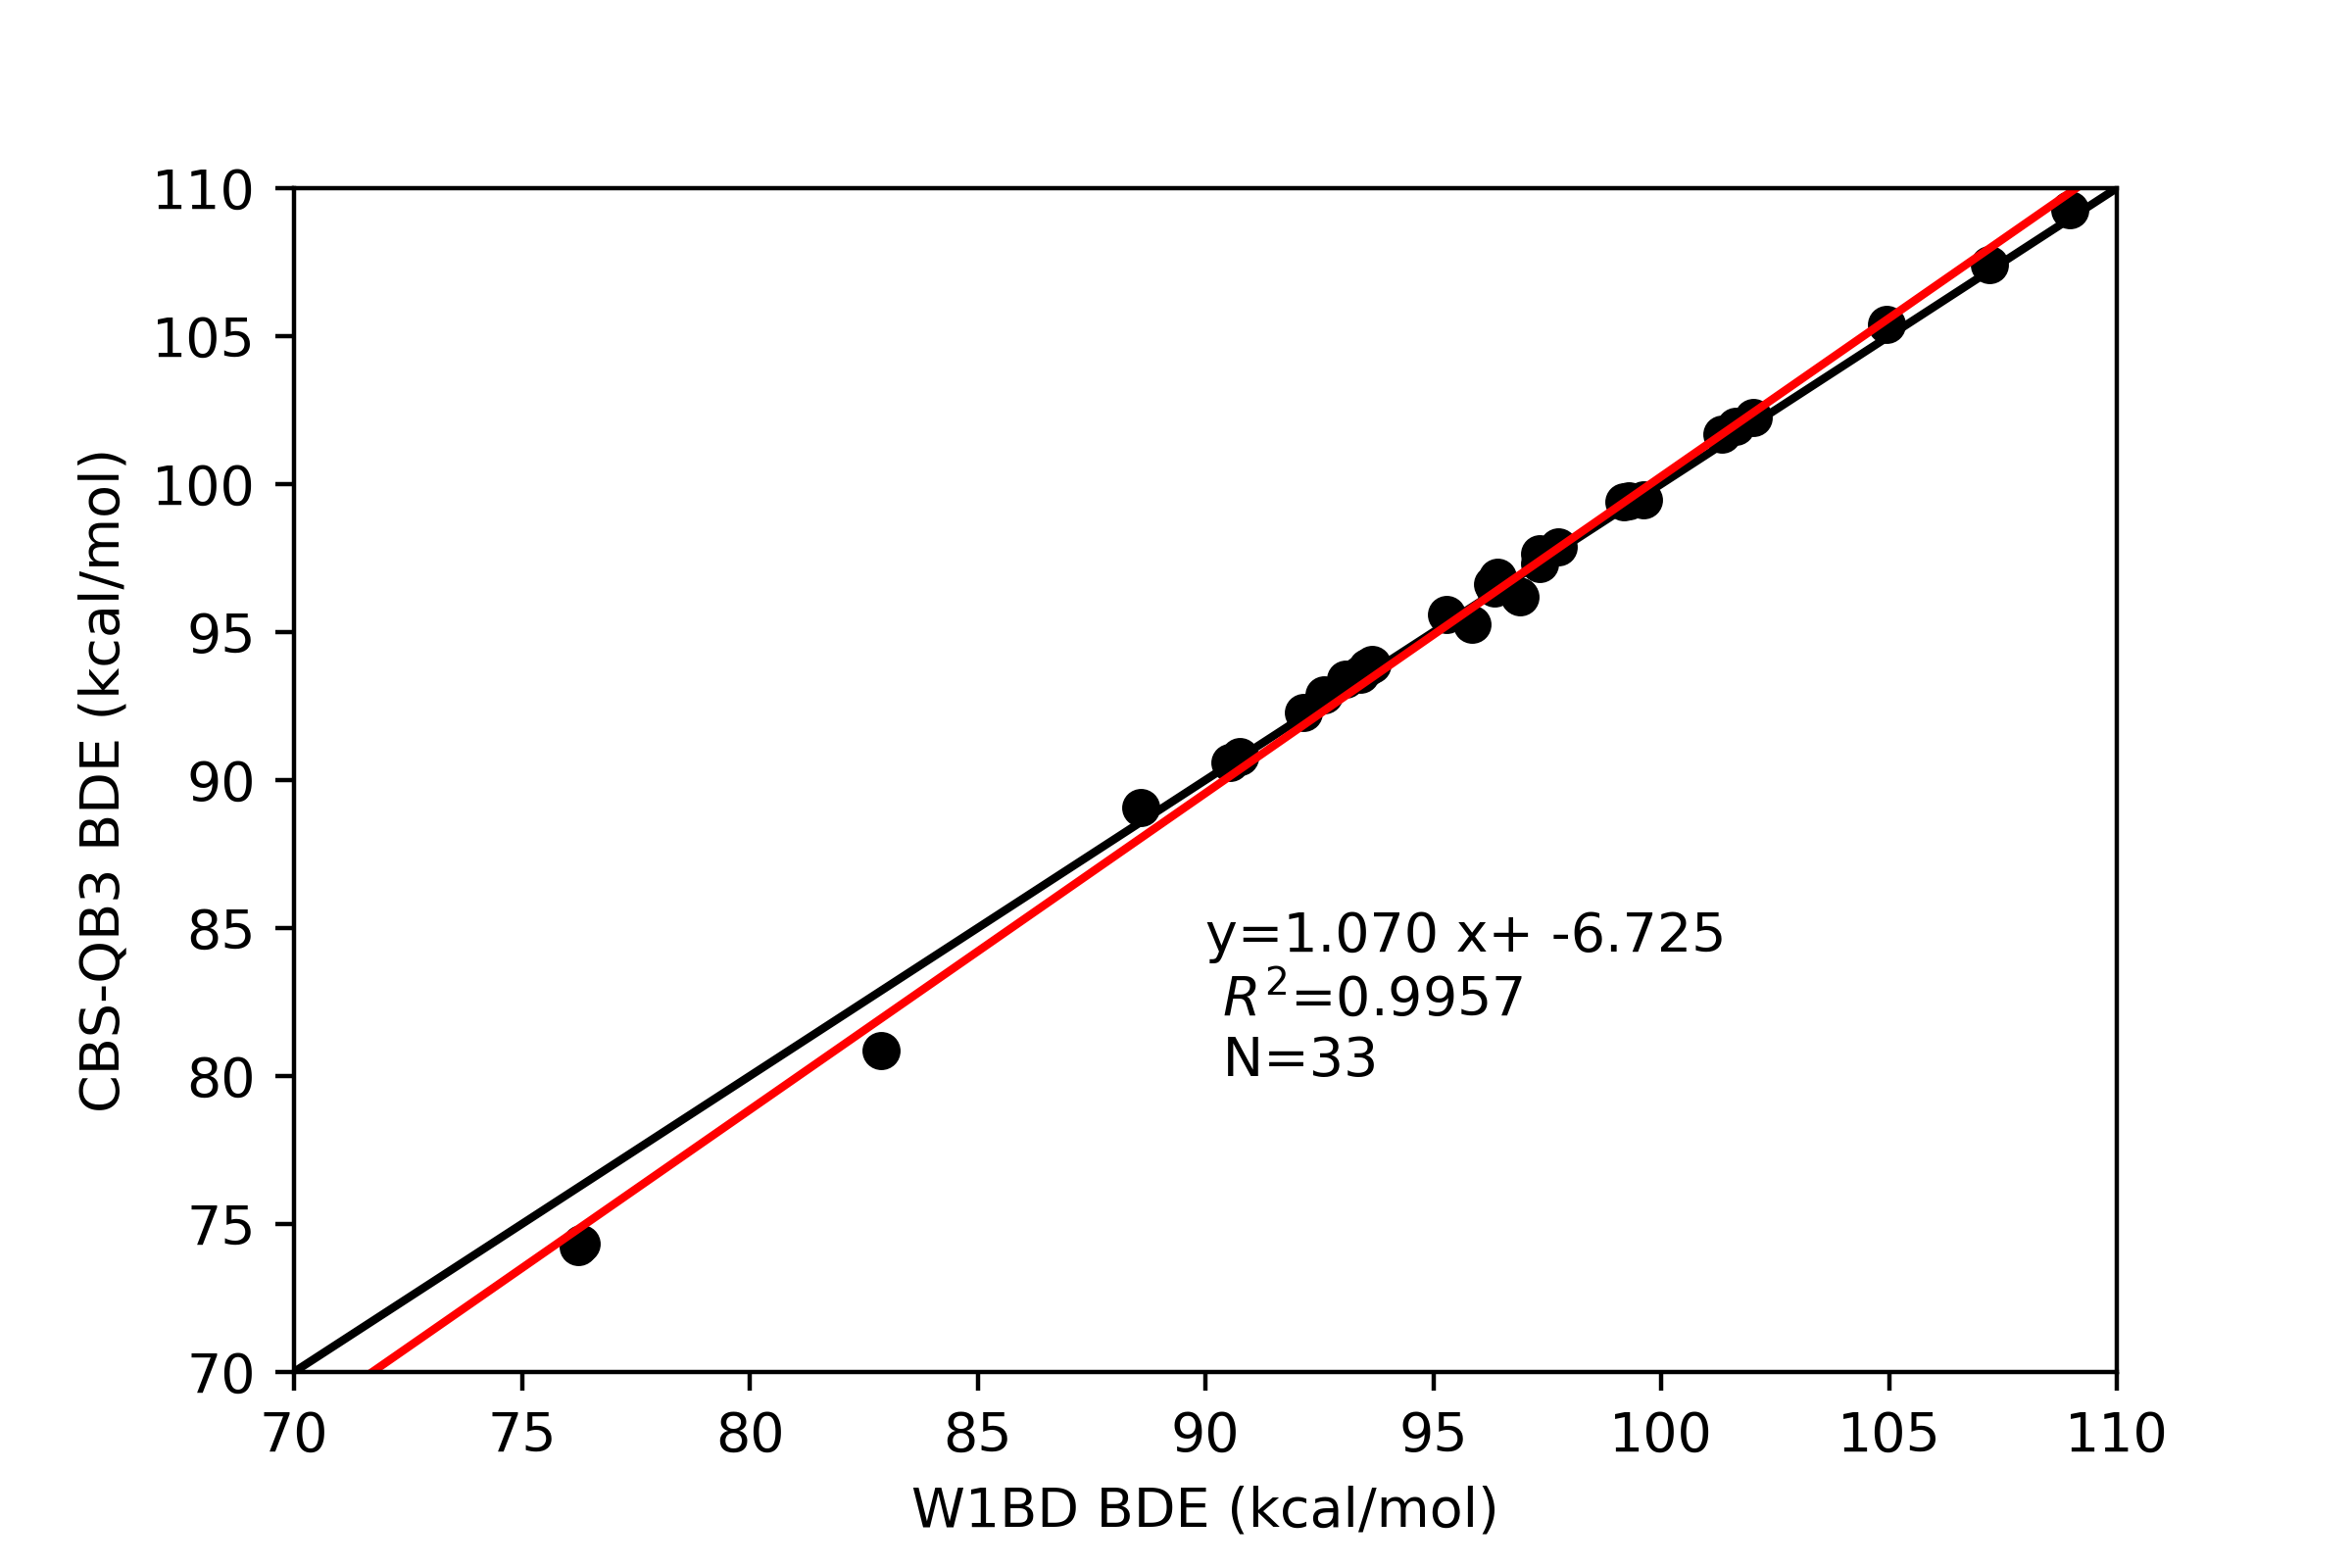
\includegraphics[width=\textwidth]{figures/w1bd-cbsqb3}
\end{minipage}%
\begin{minipage}{8cm}
  \centering
  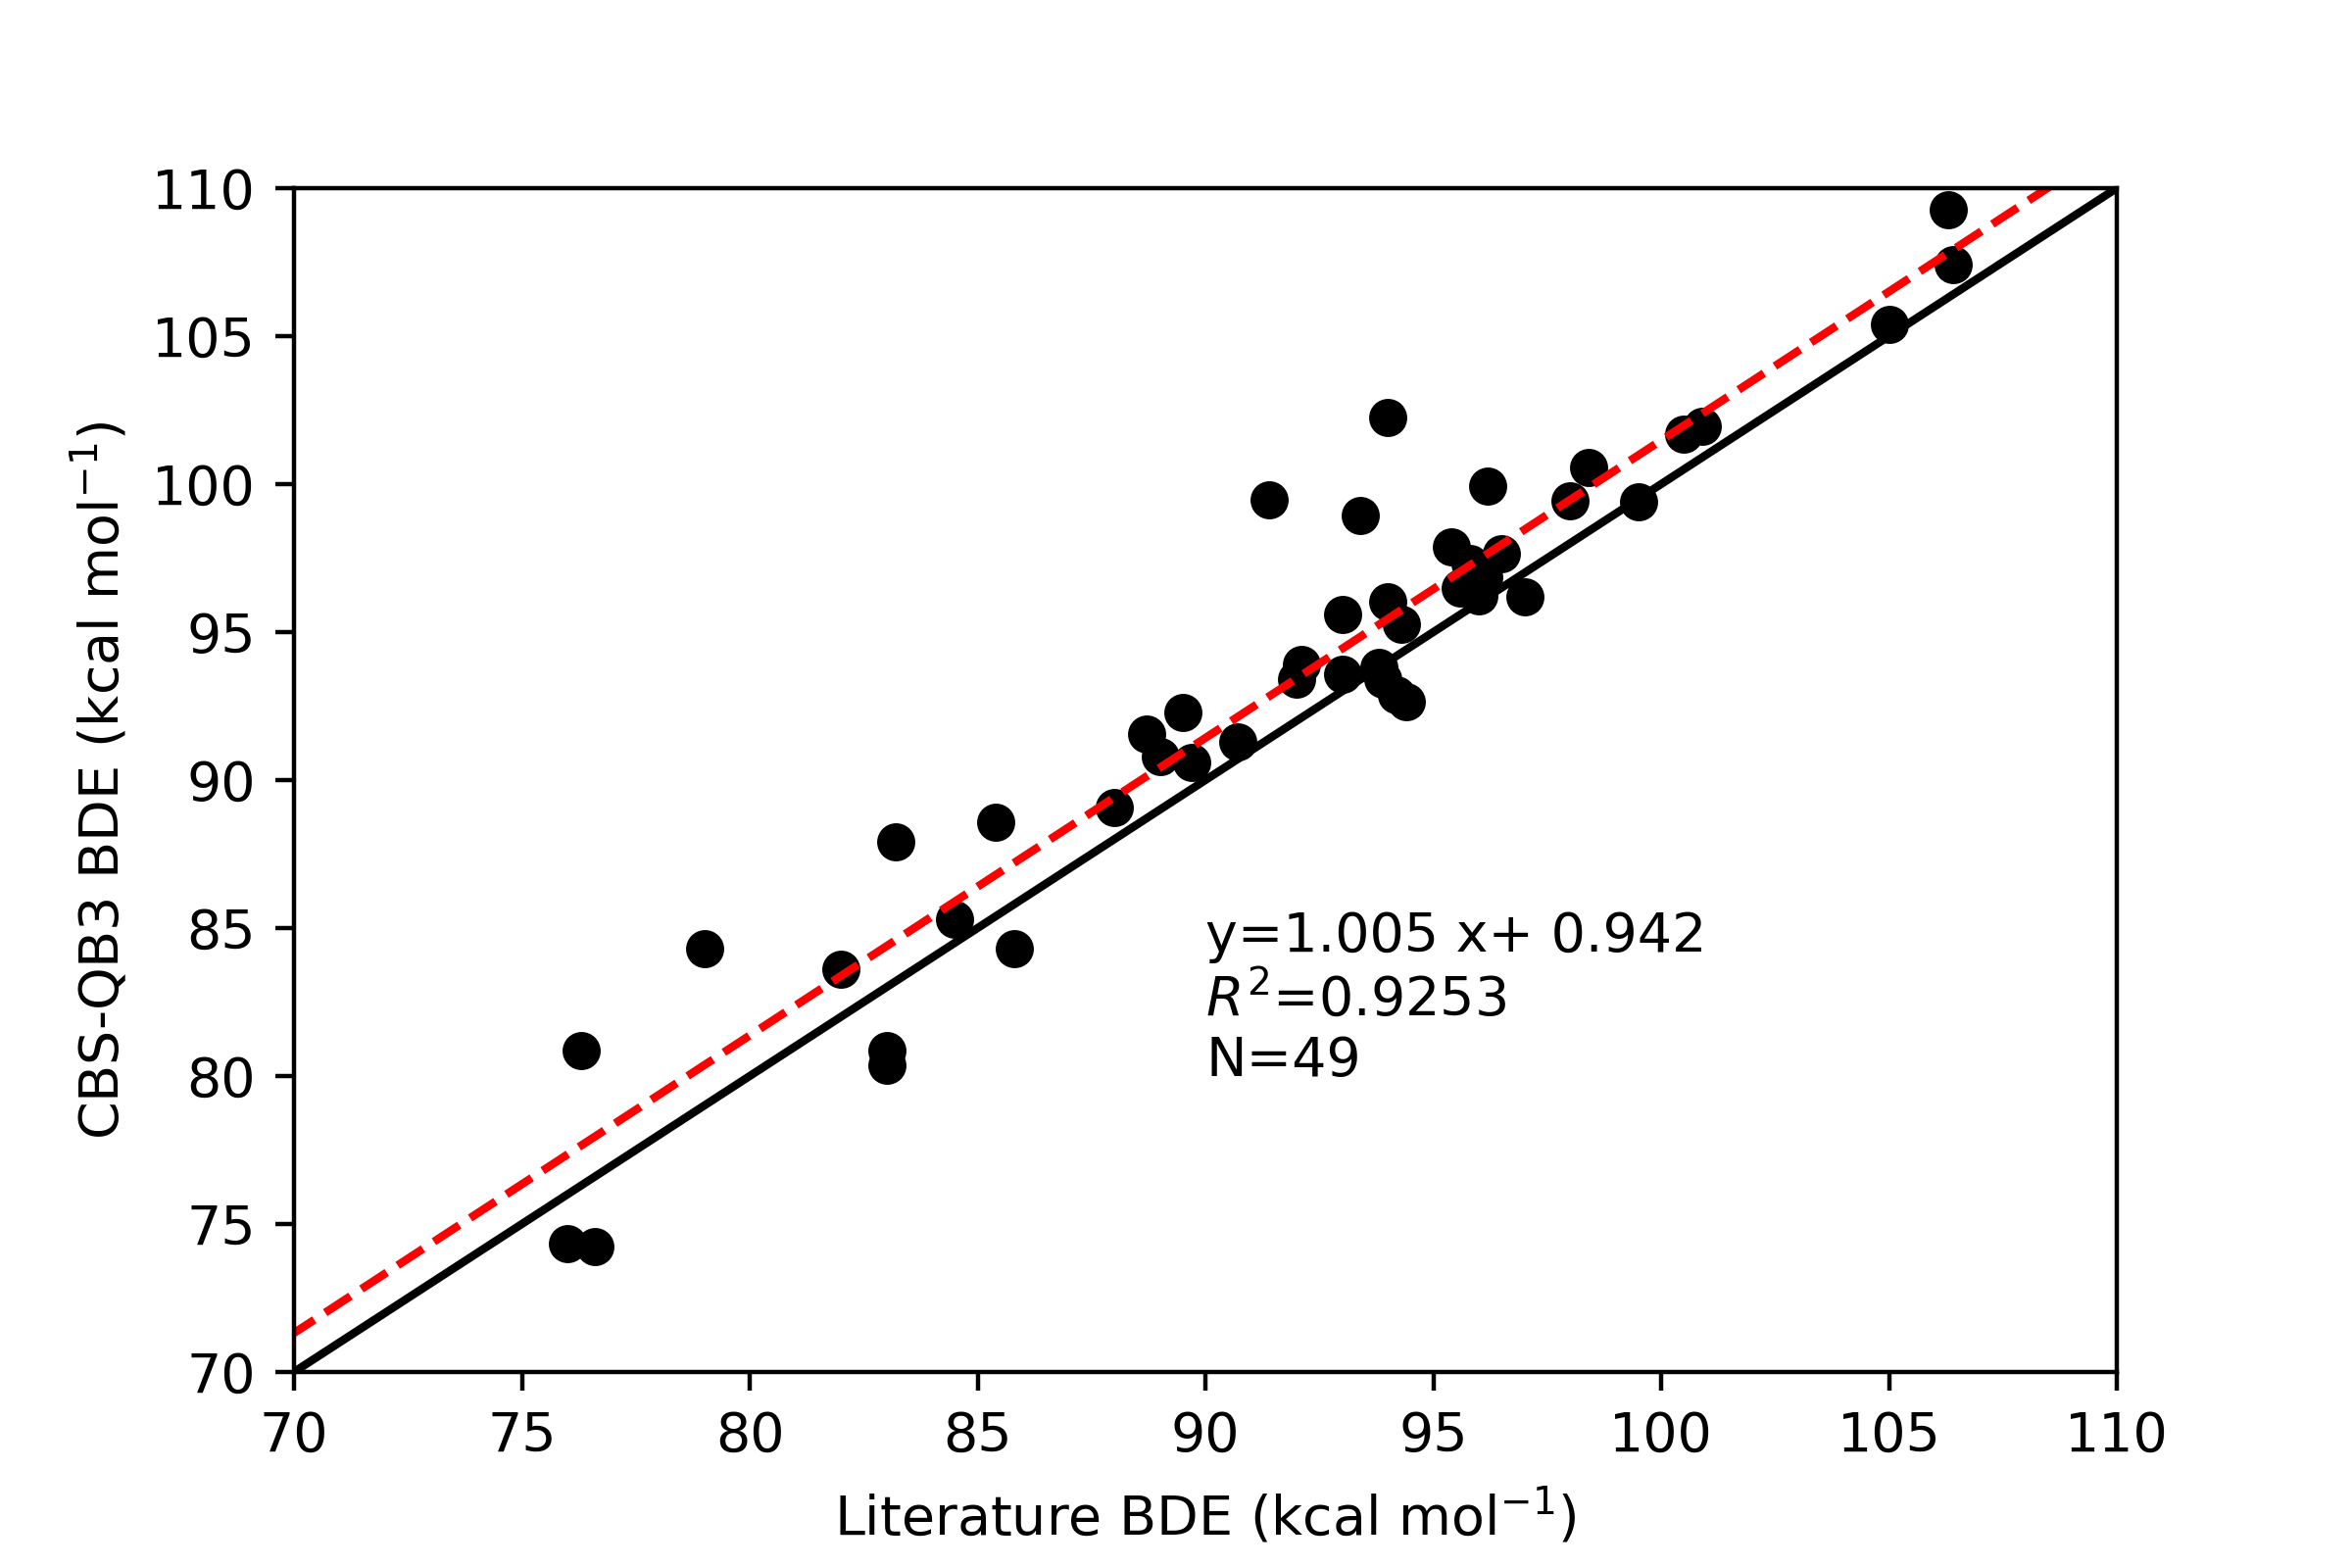
\includegraphics[width=\textwidth]{figures/lit-cbsqb3}
\end{minipage}
\caption{One-to-one plots of composite methods compared to literature and W1BD.}
\end{figure}

\begin{figure}[H]\ContinuedFloat
\hspace*{-1.8cm}
\begin{minipage}{8cm}
  \centering
  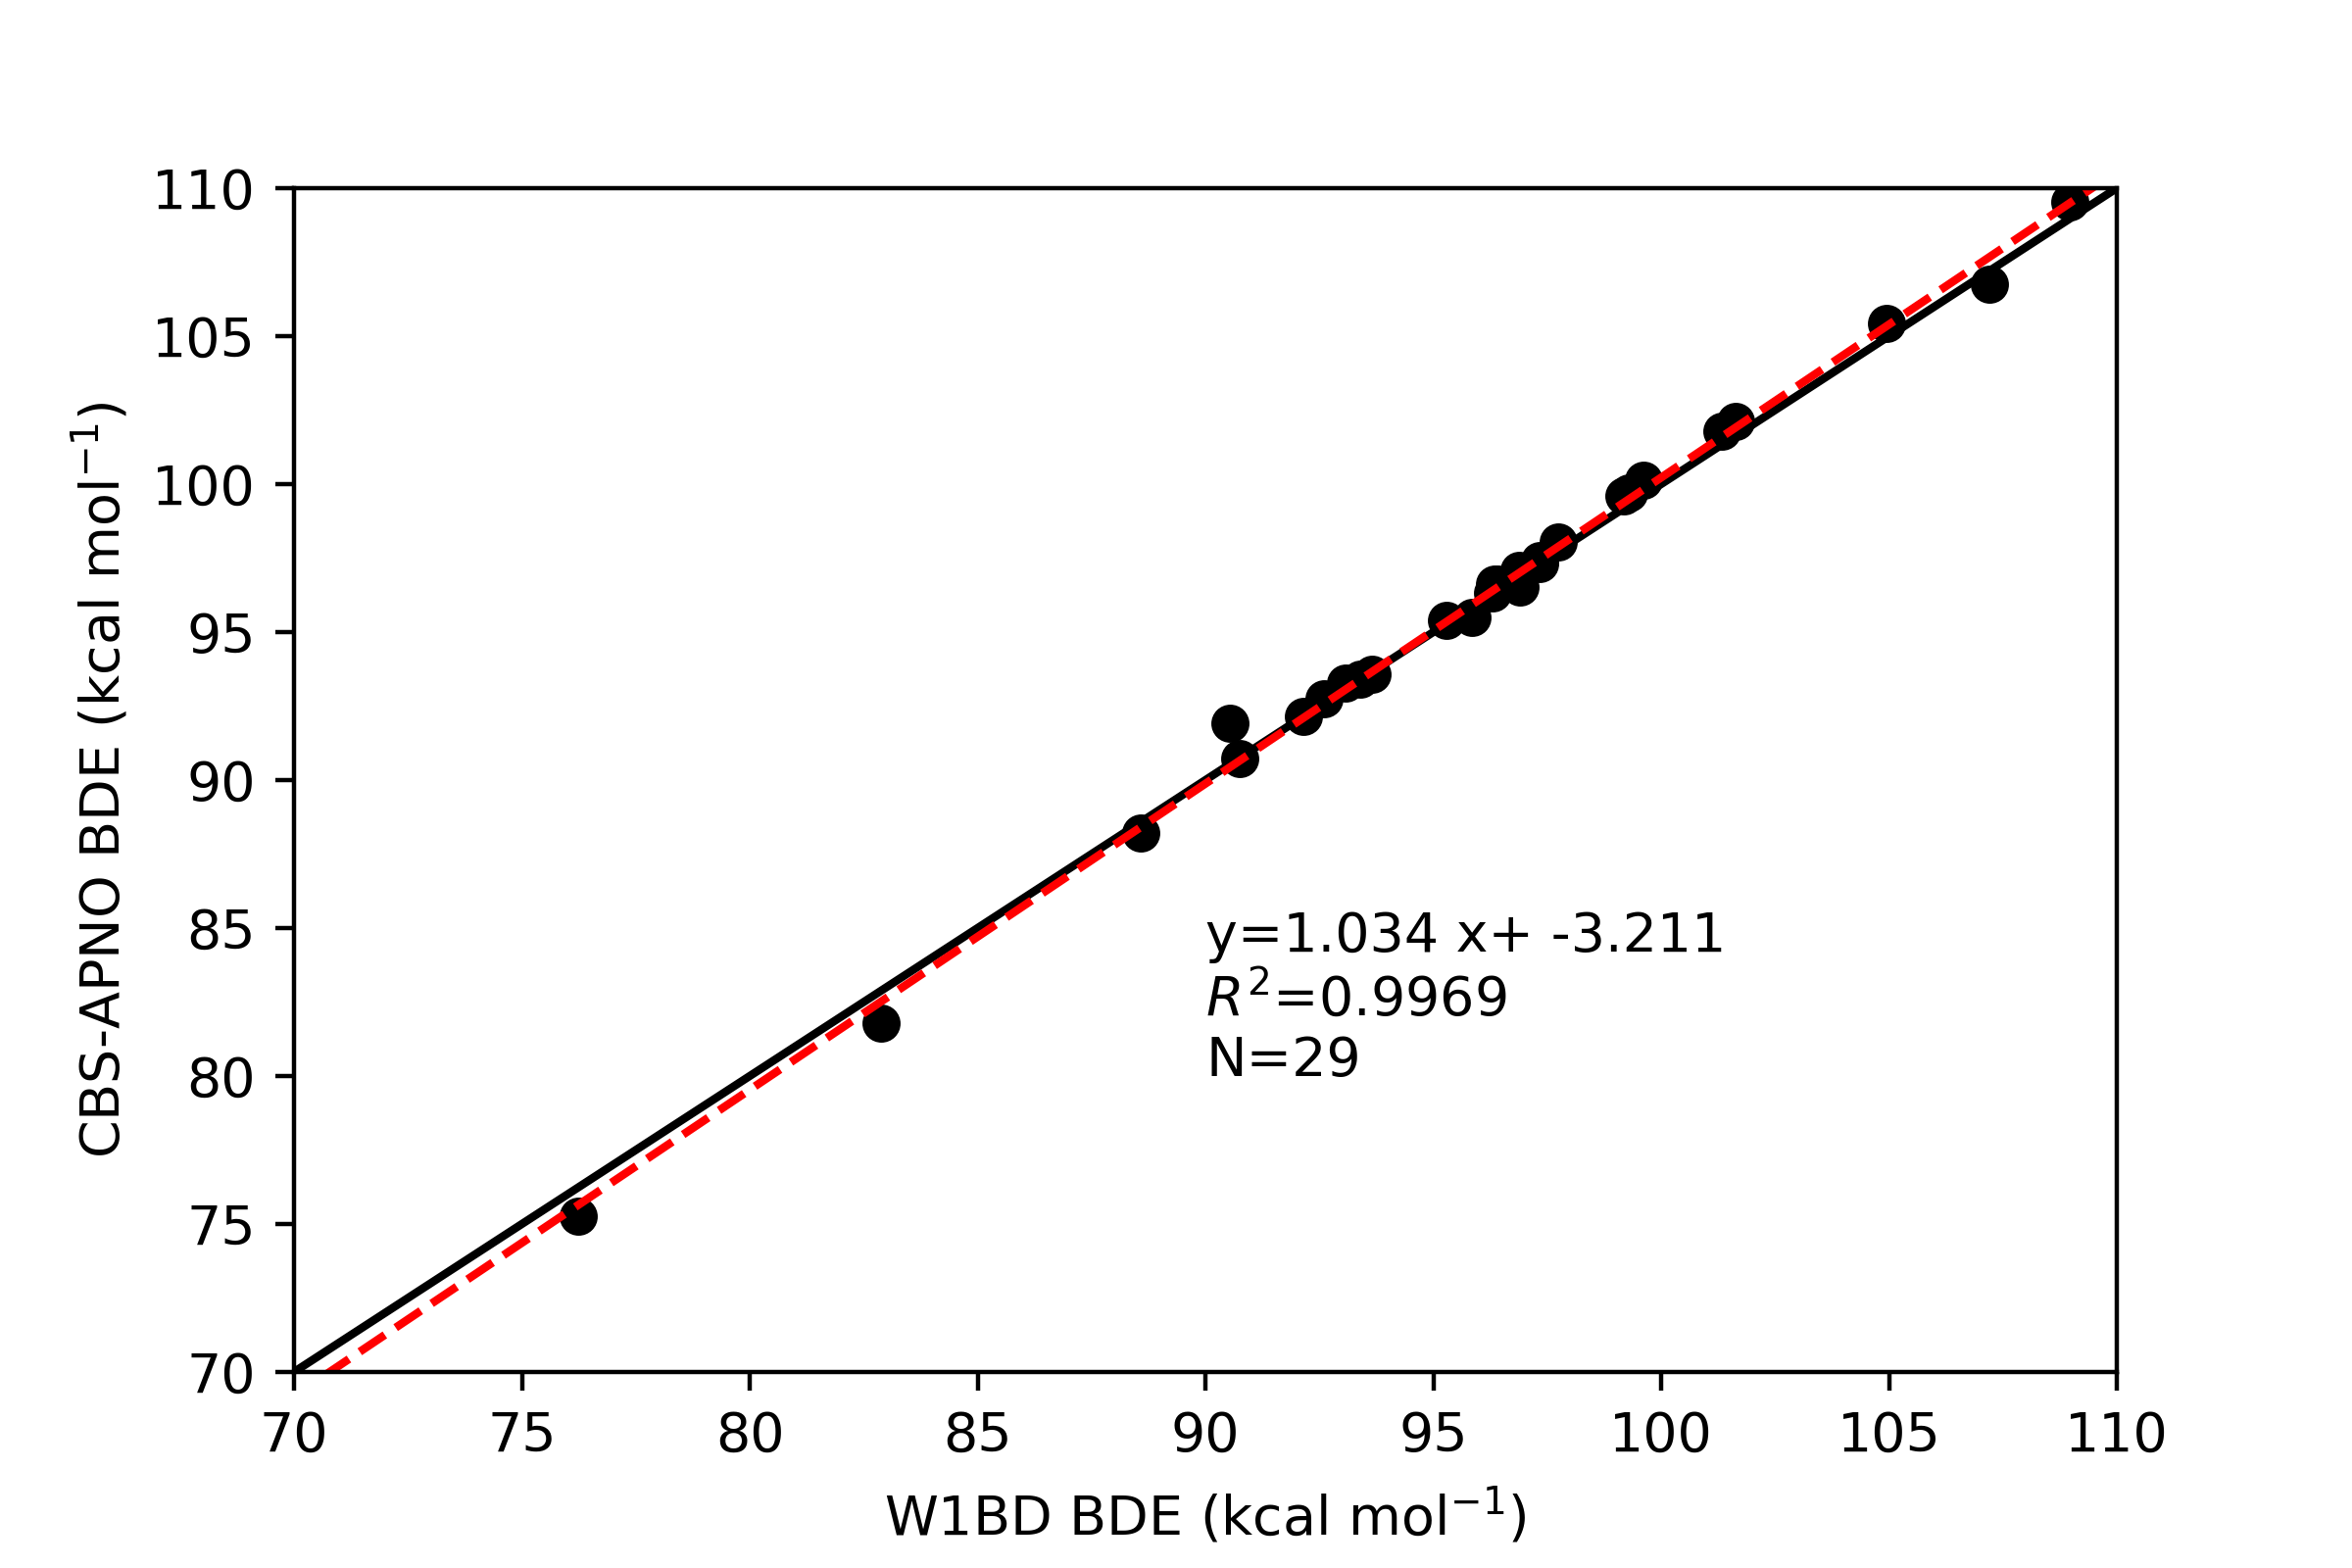
\includegraphics[width=\textwidth]{figures/w1bd-cbsapno}
\end{minipage}%
\begin{minipage}{8cm}
  \centering
  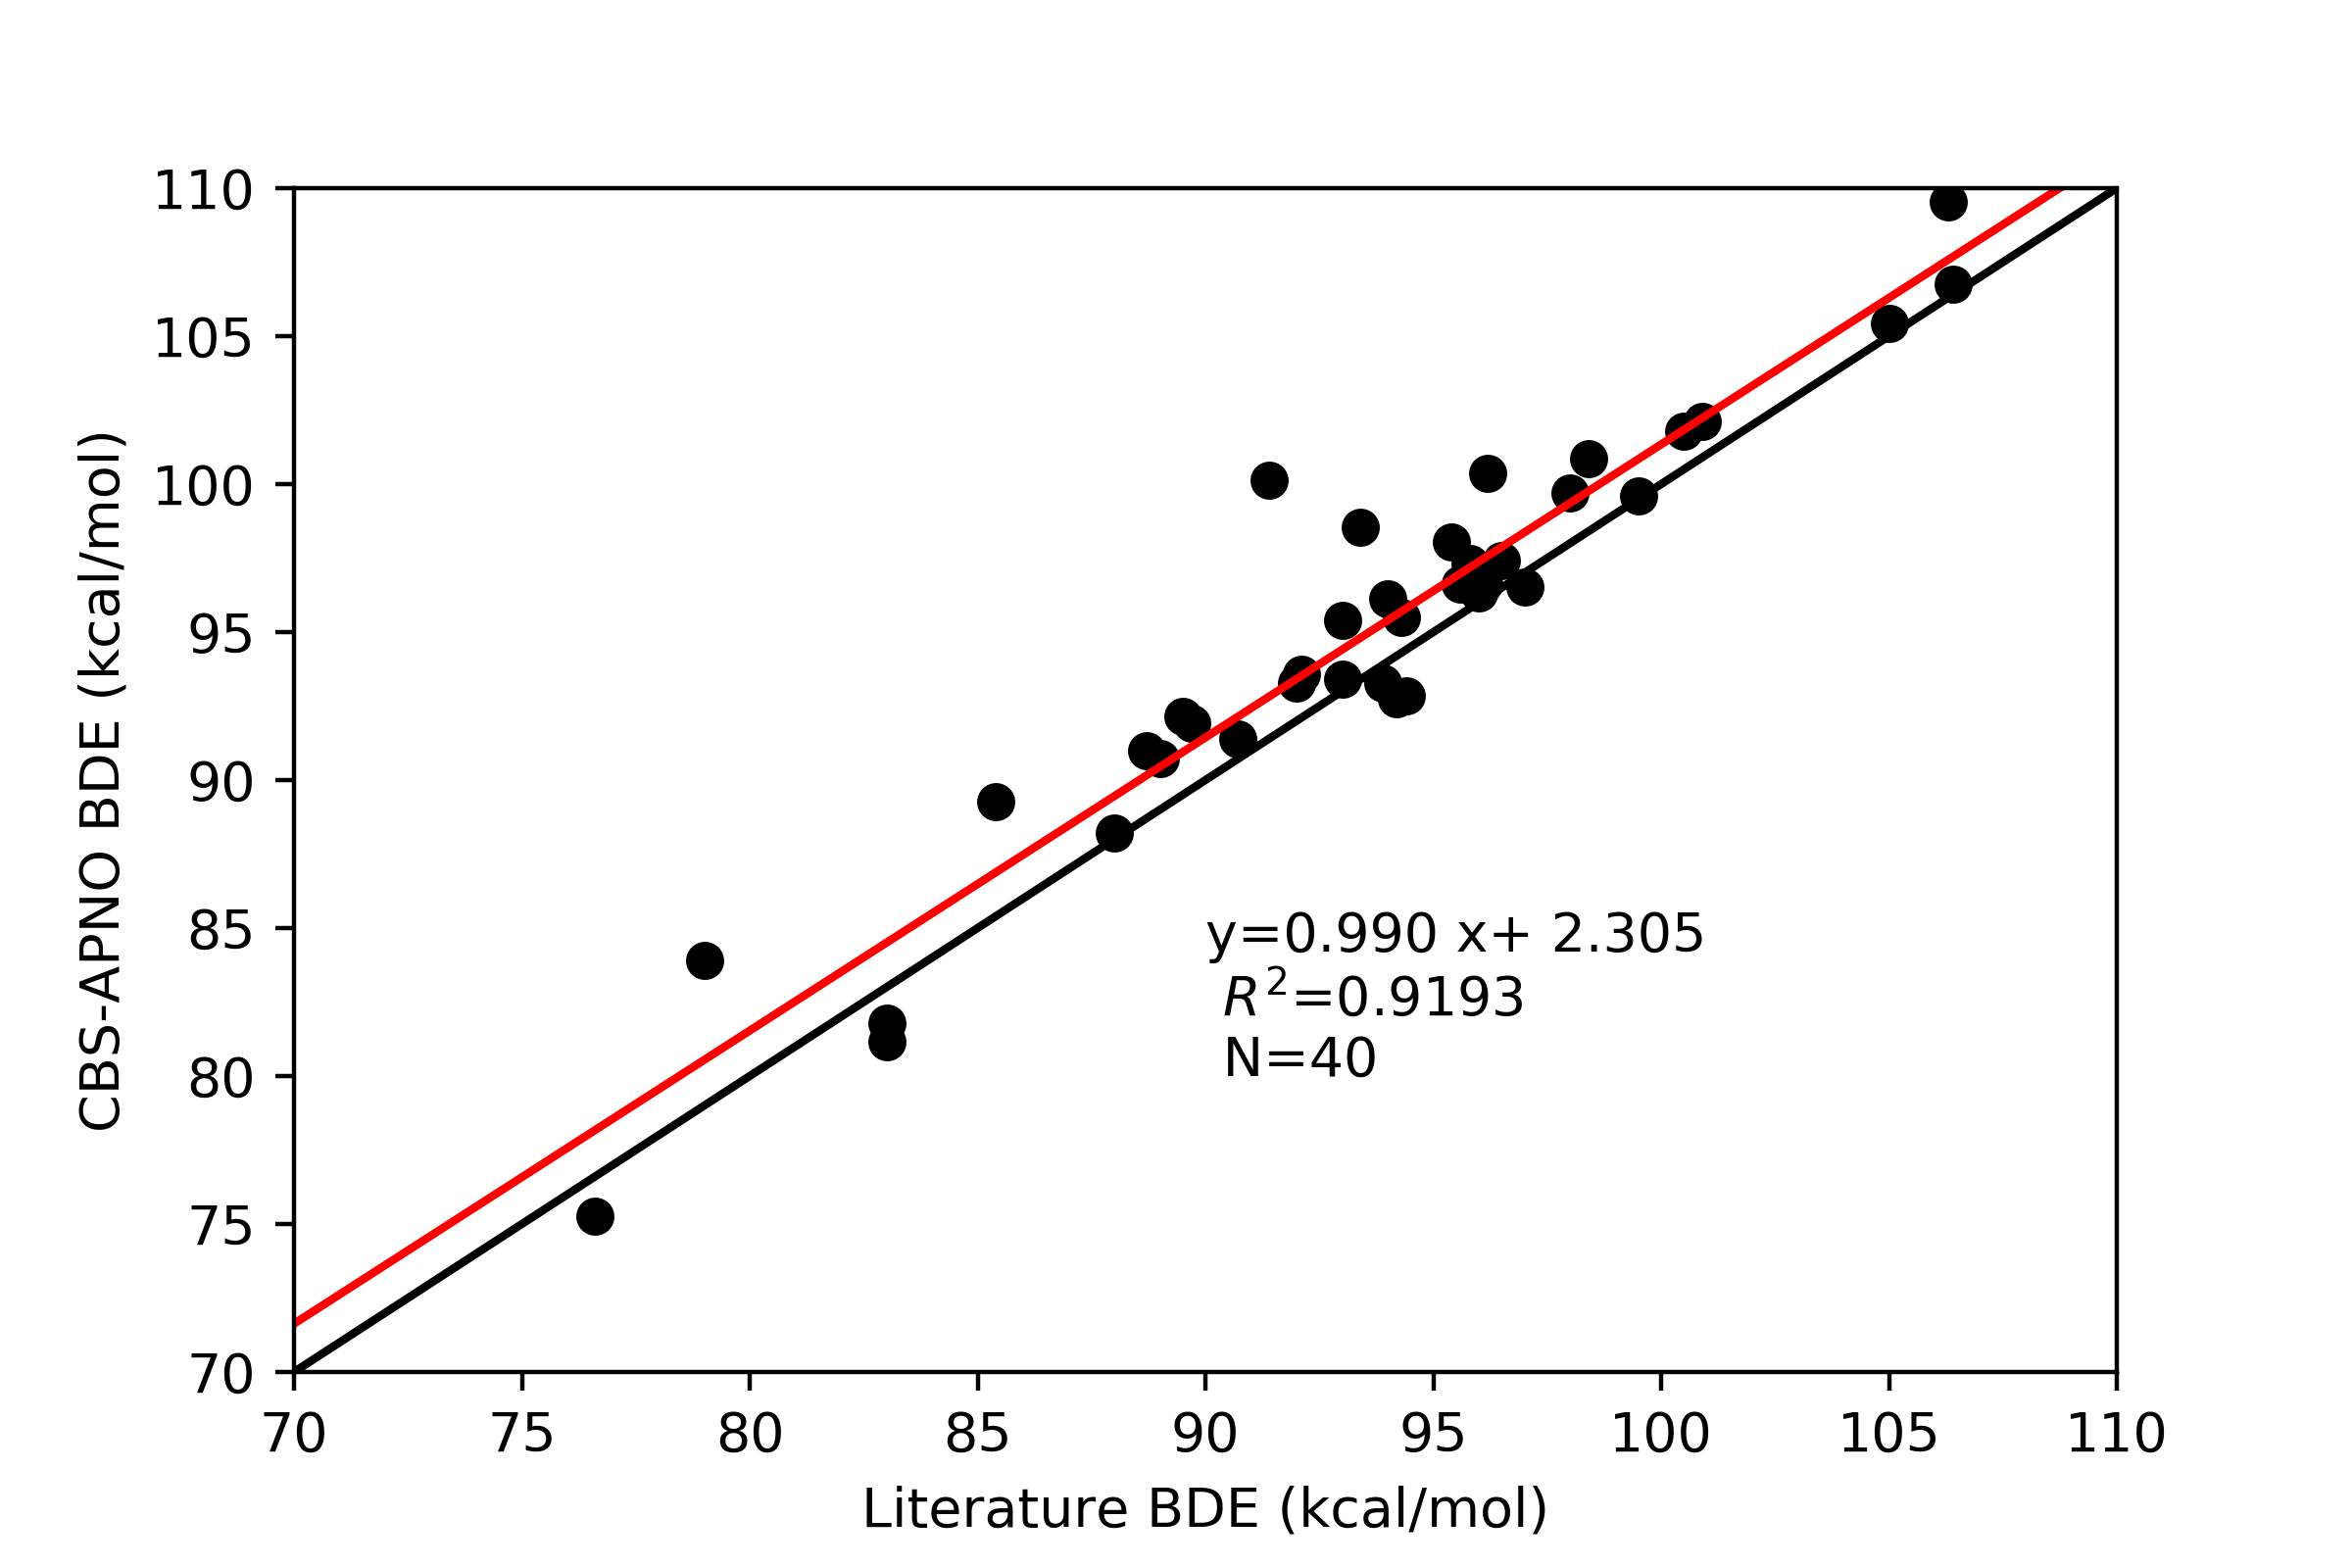
\includegraphics[width=\textwidth]{figures/lit-cbsapno}
\end{minipage}

\hspace*{-1.8cm}
\begin{minipage}{8cm}
  \centering
  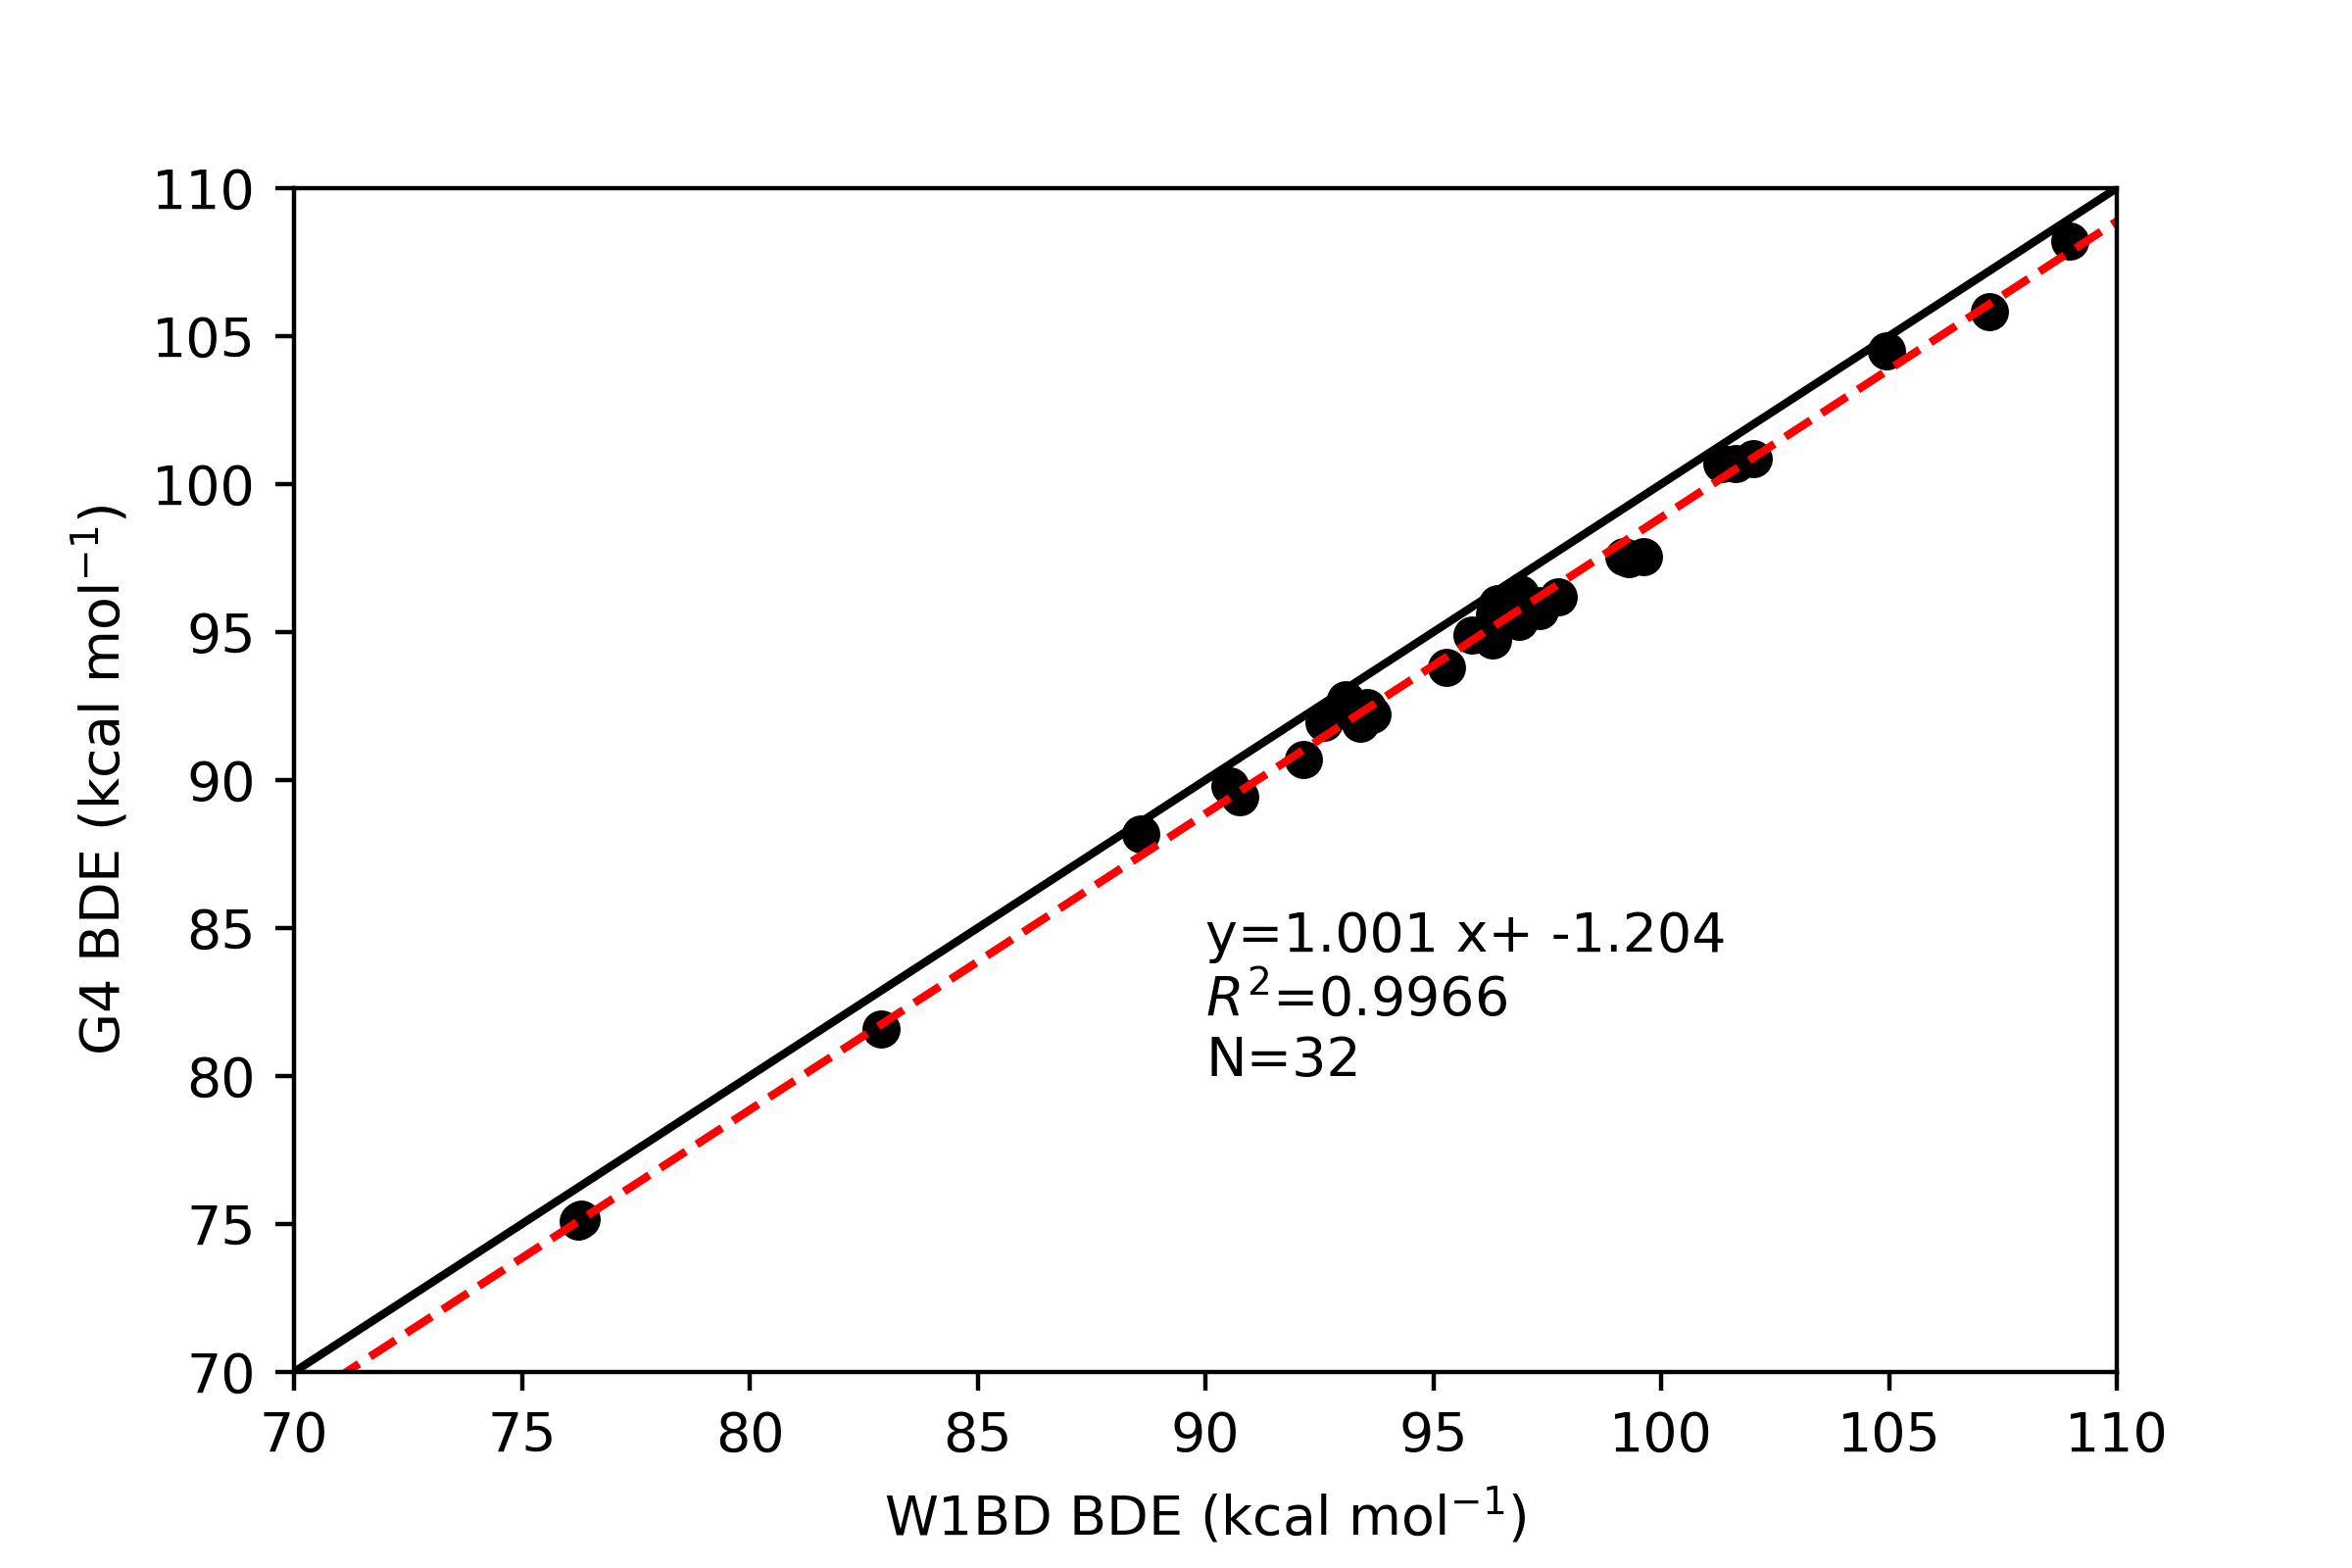
\includegraphics[width=\textwidth]{figures/w1bd-g4}
\end{minipage}%
\begin{minipage}{8cm}
  \centering
  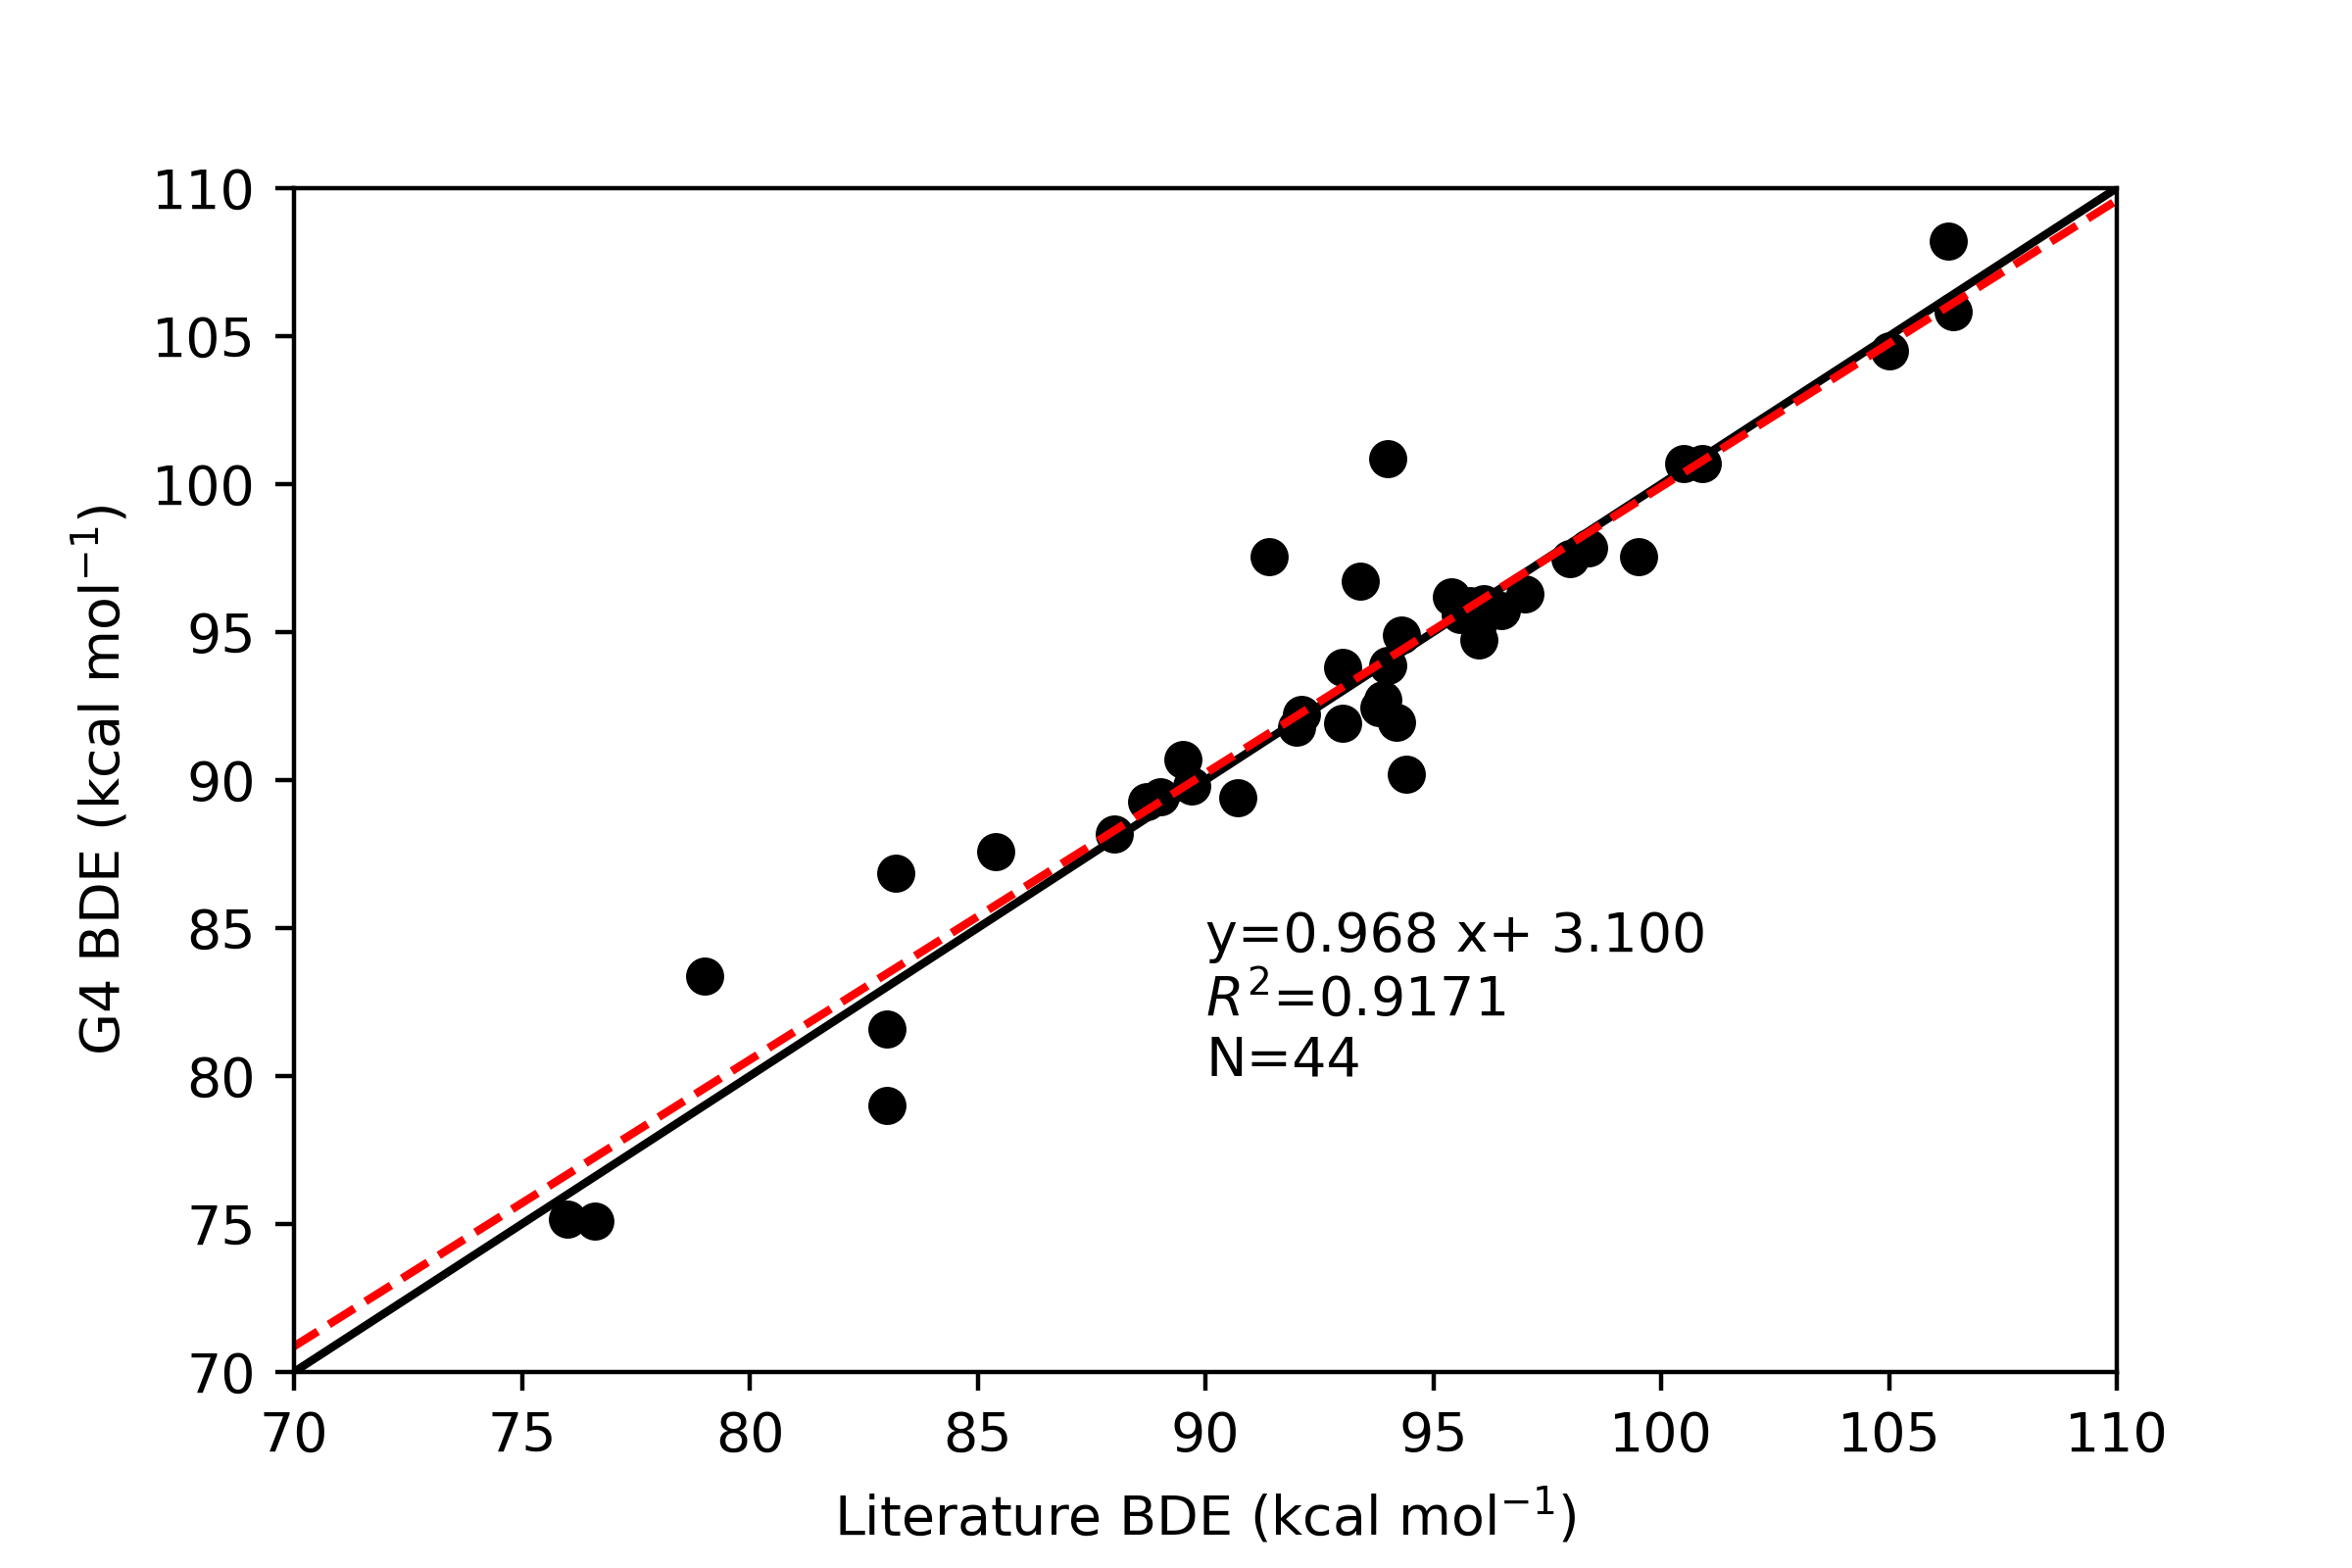
\includegraphics[width=\textwidth]{figures/lit-g4}
\end{minipage}
\caption{Continued: One-to-one plots of composite methods compared to literature and W1BD.}
\end{figure}

\begin{figure}[H]\ContinuedFloat
\hspace*{-1.8cm}
\begin{minipage}{8cm}
  \centering
  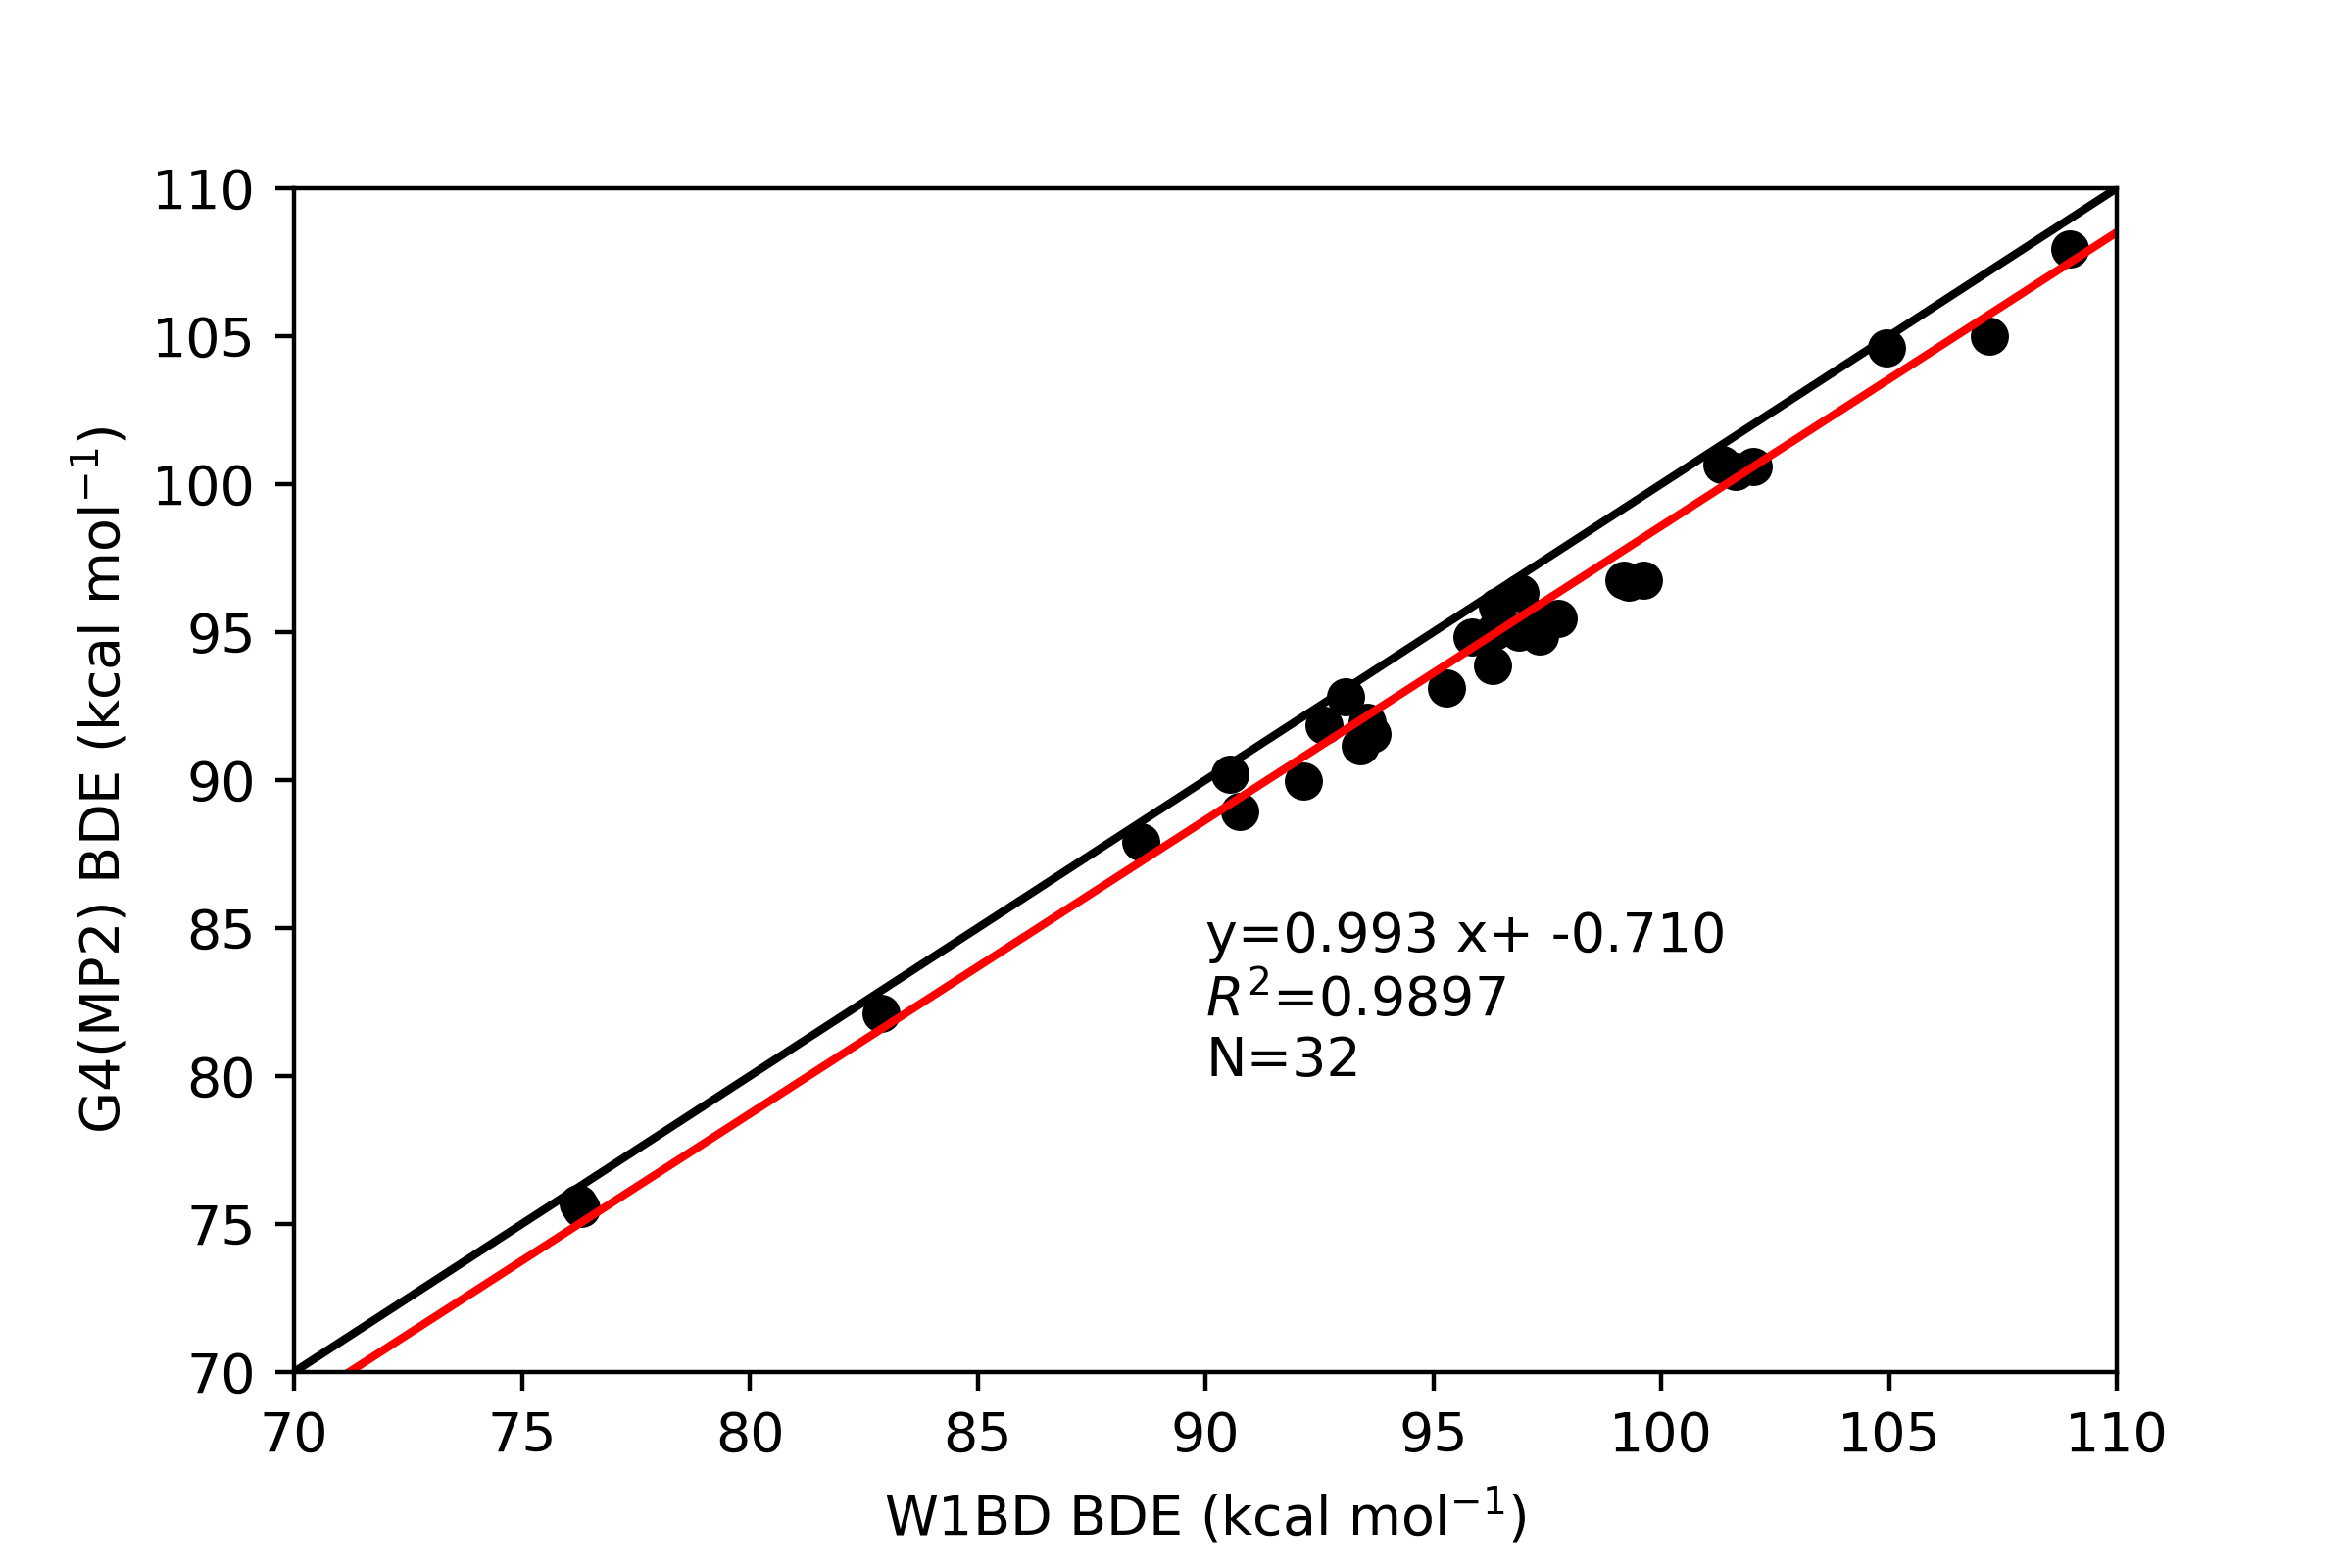
\includegraphics[width=\textwidth]{figures/w1bd-g4mp2}
\end{minipage}%
\begin{minipage}{8cm}
  \centering
  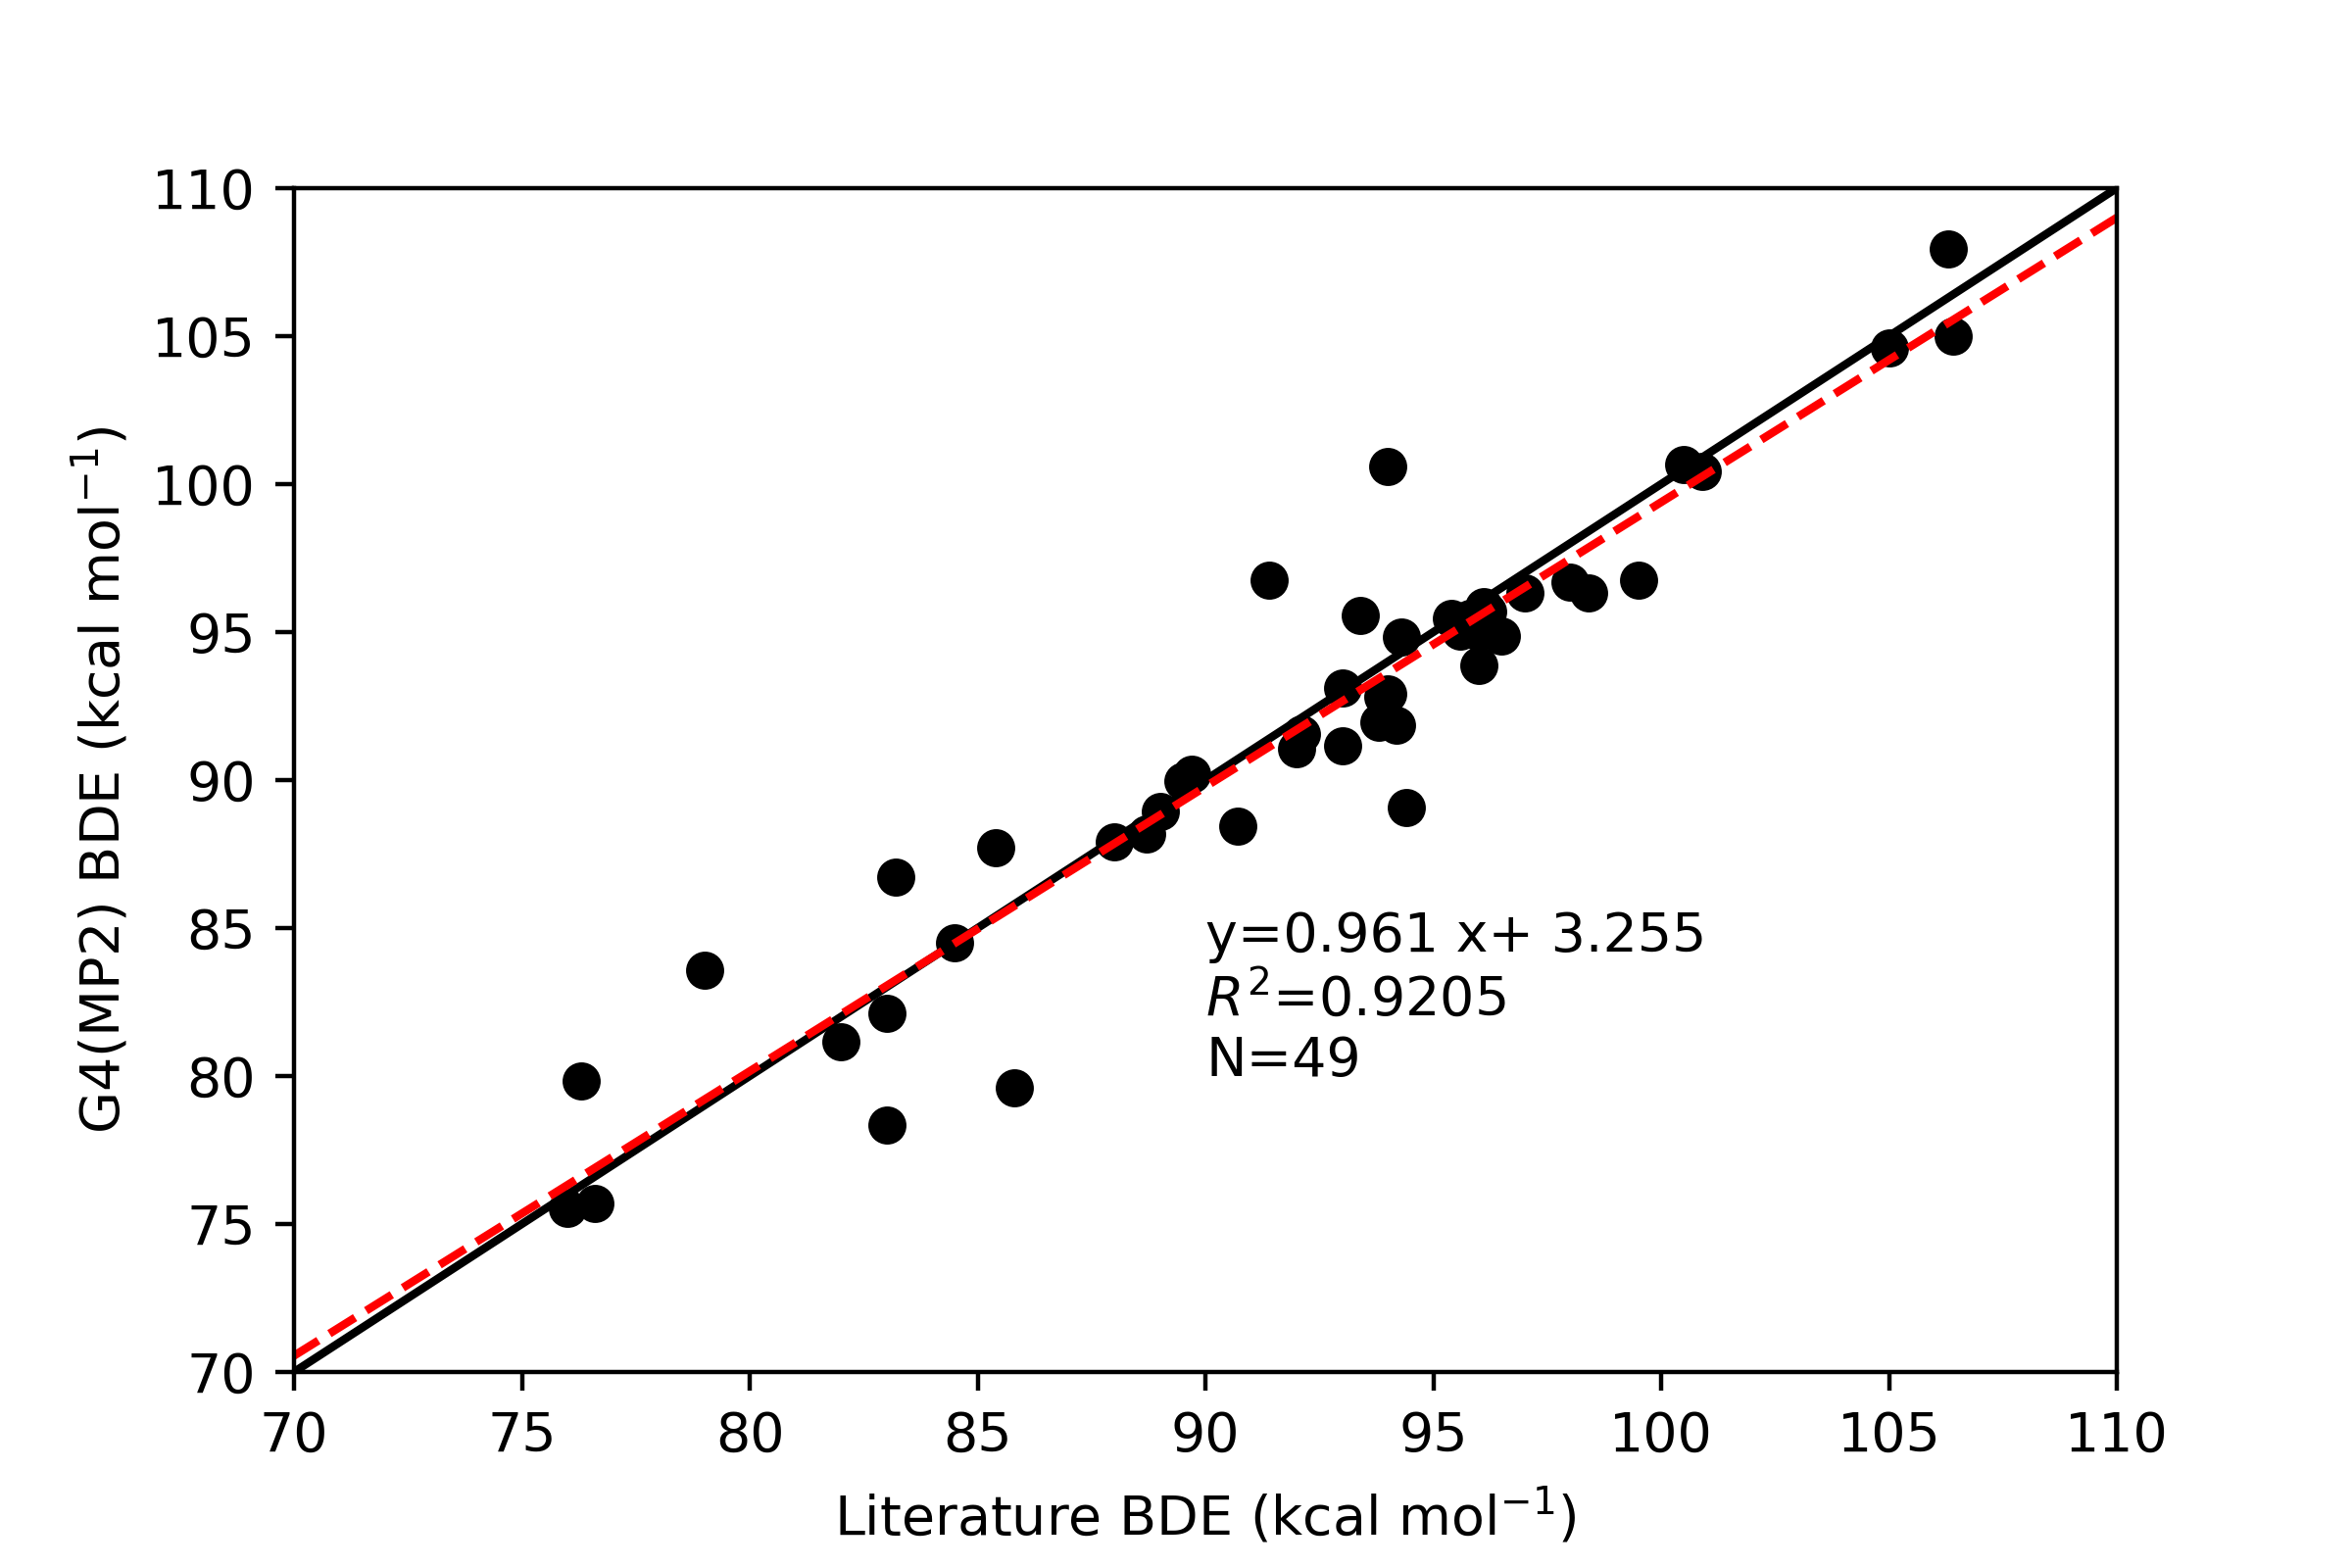
\includegraphics[width=\textwidth]{figures/lit-g4mp2}
\end{minipage}
\caption{Continued: One-to-one plots of composite methods compared to literature and W1BD.}
\end{figure}

\begin{longtable}{m{3.1cm} | c c c}
\caption[Summary of experimental rate constants and literature bond dissociation enthalpies (BDEs).]{Summary of experimental rate constants and literature\cite{Luo2002} bond dissociation enthalpies (BDEs).} \label{tab:expt-bde} \\
\centering
 Molecule                       & $k_H$ \Ms          & Normalized $k_H$ \Ms & BDE \kcalmol \\
\toprule
 1,4-cyclohexadiene             & $ 6.60 \times 10^7$ & $1.65 \times 10^7 $ &        76 \\
 1,4-diazabicyclo-[2.2.2]octane  & $ 9.60 \times 10^6$ & $8.00 \times 10^5 $ &      93.4 \\
 2,2-dimethylbutane             & $ 9.50 \times 10^4$ & $4.75 \times 10^4 $ &        98 \\
 2,3-dimethylbutane             & $ 5.60 \times 10^5$ & $2.80 \times 10^5 $ &      95.4 \\
 9,10-dihydroanthracene         & $ 5.04 \times 10^7$ & $1.26 \times 10^7 $ &      76.3 \\
 Acetone                        & $ < 1 \times 10^4 $ & $2 \times 10^3    $ &        96 \\
 Acetonitrile                   & $ < 1 \times 10^4 $ & $2 \times 10^3    $ &        97 \\
 Adamantane (2$^\circ$)                & $ 6.90 \times 10^6$ & $5.75 \times 10^5 $ &      98.4 \\
 Adamantane (3$^\circ$)                & $ 6.90 \times 10^6$ & $1.73 \times 10^6 $ &      96.2 \\
 Benzaldehyde                   & $ 1.20 \times 10^7$ & $1.20 \times 10^7 $ &      88.7 \\
 Benzyl alcohol                 & $ 2.97 \times 10^6$ & $1.49 \times 10^6 $ &        79 \\
 Cumene                         & $ 5.60 \times 10^5$ & $5.60 \times 10^5 $ &      83.2 \\
 Cycloheptane                   & $ 2.20 \times 10^6$ & $1.57 \times 10^5 $ &        94 \\
 Cyclohexane                    & $ 1.10 \times 10^6$ & $9.17 \times 10^4 $ &      99.5 \\
 Cyclooctane                    & $ 2.98 \times 10^6$ & $1.86 \times 10^5 $ &      94.4 \\
 Cyclopentane                   & $ 9.54 \times 10^6$ & $9.54 \times 10^5 $ &      95.6 \\
 Dibenzyl ether                 & $ 5.60 \times 10^6$ & $1.40 \times 10^6 $ &      85.8 \\
 Diethyl ether                  & $ 2.60 \times 10^6$ & $6.50 \times 10^5 $ &        93 \\
 Dimethyl sulfoxide              & $ 1.80 \times 10^4$ & $6.00 \times 10^3 $ &        94 \\
 Dioxane                        & $ 8.20 \times 10^5$ & $1.03 \times 10^5 $ &      96.5 \\
 Diphenylmethane                & $ 8.71 \times 10^5$ & $4.36 \times 10^5 $ &      84.5 \\
 Ethylbenzene                   & $ 7.90 \times 10^5$ & $3.95 \times 10^5 $ &      85.4 \\
 Hexamethyl-phorsphoramide       & $ 1.87 \times 10^7$ & $1.04 \times 10^6 $ &           \\
 Morpholine                     & $ 5.00 \times 10^7$ & $1.25 \times 10^7 $ &        92 \\
 Piperazine                     & $ 2.4 \times 10^8 $ &                &        93 \\
 Piperidine                     & $ 1.2 \times 10^8 $ &                &      89.5 \\
 Pyrrolidine                    & $ 1.1 \times 10^8 $ &                &        89 \\
 Tetrahydro-2H-pyran            & $ 1.4 \times 10^6 $ &                &        96 \\
 Tetrahydrofuran                & $ 5.8 \times 10^6 $ &                &      92.1 \\
 Toluene                        & $ 1.85 \times 10^5$ & $6.17 \times 10^4 $ &      89.7 \\
 Triethylamine                  & $ 2.10 \times 10^8$ & $3.5 \times 10^7  $ &      90.7 \\
 Triphenylmethane               & $ 3.04 \times 10^5$ & $3.04 \times 10^5 $ &        81 \\
\end{longtable}


\chapter{Chapter~\protect\ref{ch:hat} Additional Data}\label{ap:hat}

\begin{scheme}[!htbp]
  \centering
    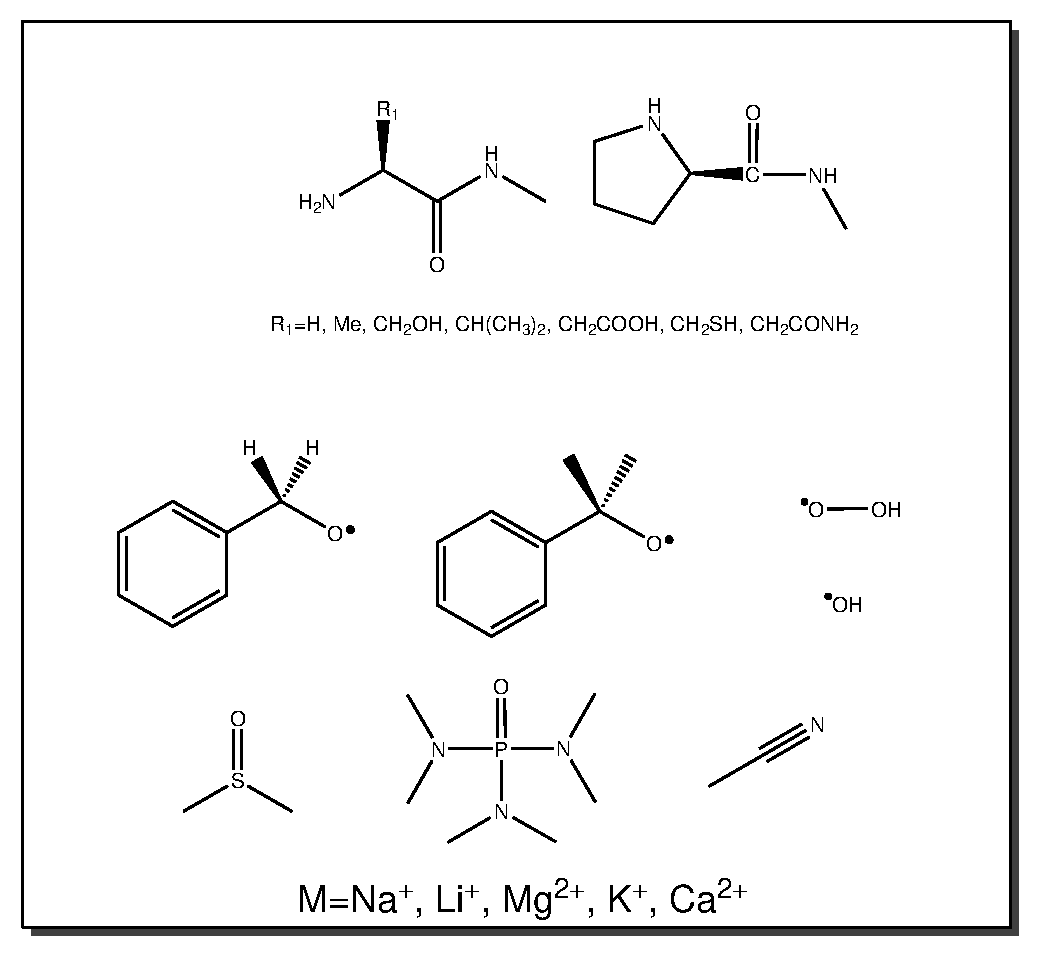
\includegraphics[width=\textwidth]{figures/set1.eps}
    \caption[Initial proposed benchmark set of substrates/radicals and metal cations.]{Initial proposed benchmark set of substrates/radicals and metal cations. Note this set consists of all combinations of substrates and metal cation, thus there are 75 complexes in the set. Conformational analysis using the Hyperchem package\cite{Hyperchem16} to identify the lowest energy conformers of all the substrates was completed using the AM1 semi-empirical approach. Geometry optimizations were then performed without metal cations at the LC-$\omega$PBE-D3(BJ)/6-31+G(2d,2p) level of theory. Several binding sites were investigated and optimized at the same level of theory. Benchmark quality structures have been optimized at the LC-$\omega$PBE-D3(BJ)/6-311+G(3df,3pd) level of theory. I am awaiting computational resources to performed CCSD(T)-F12$^*$/Def2-QZVPPD calculations.}
  \label{fig:ap-set1}
\end{scheme}

\begin{figure}[!htbp]
  \centering
    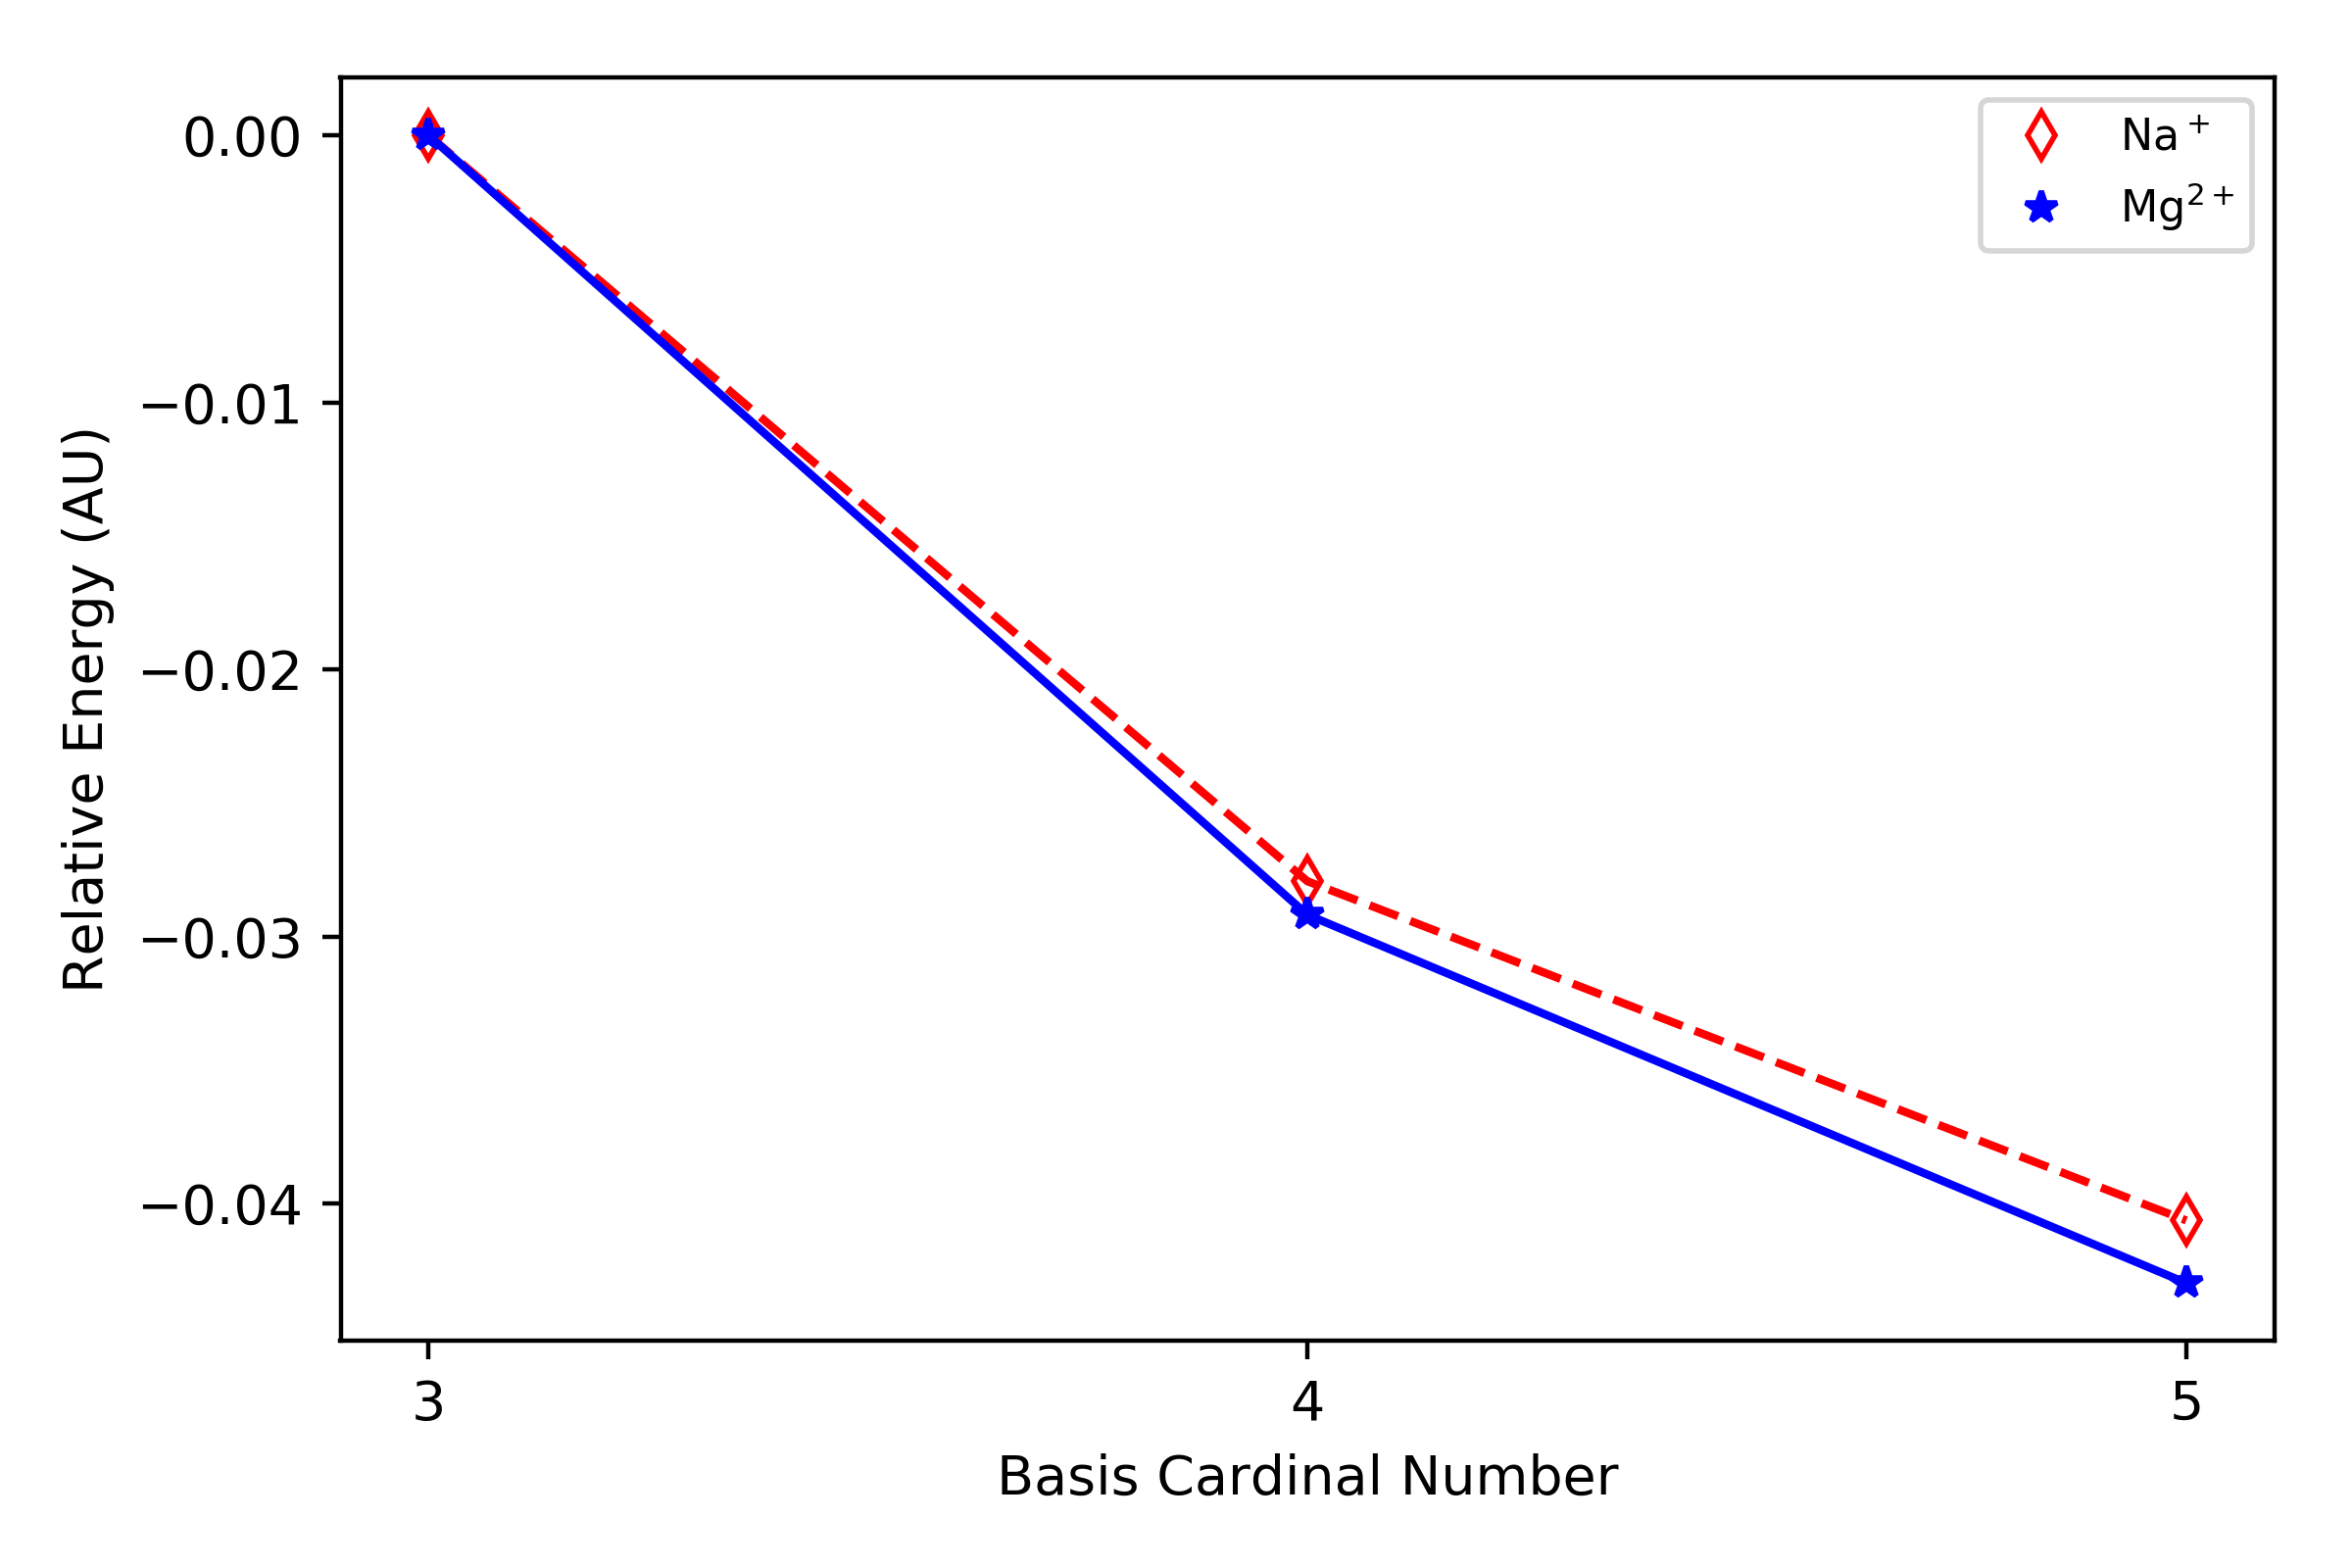
\includegraphics[width=\textwidth]{figures/ap_pes_metals}
    \caption[Basis set convergence for sodium and magnesium ions with core-correlation basis sets.]{Basis set convergence of CCSD(T,Full)/cc-pVC$X$Z ($X$=3,4,5) for sodium and magnesium ions. The relative energy of each basis set relative to the cc-pVCDZ for each metal. The cardinal number of the basis sets is $X$.}
  \label{fig:ap_pes_metals}
\end{figure}



\begin{figure}[!htbp]
  \centering
    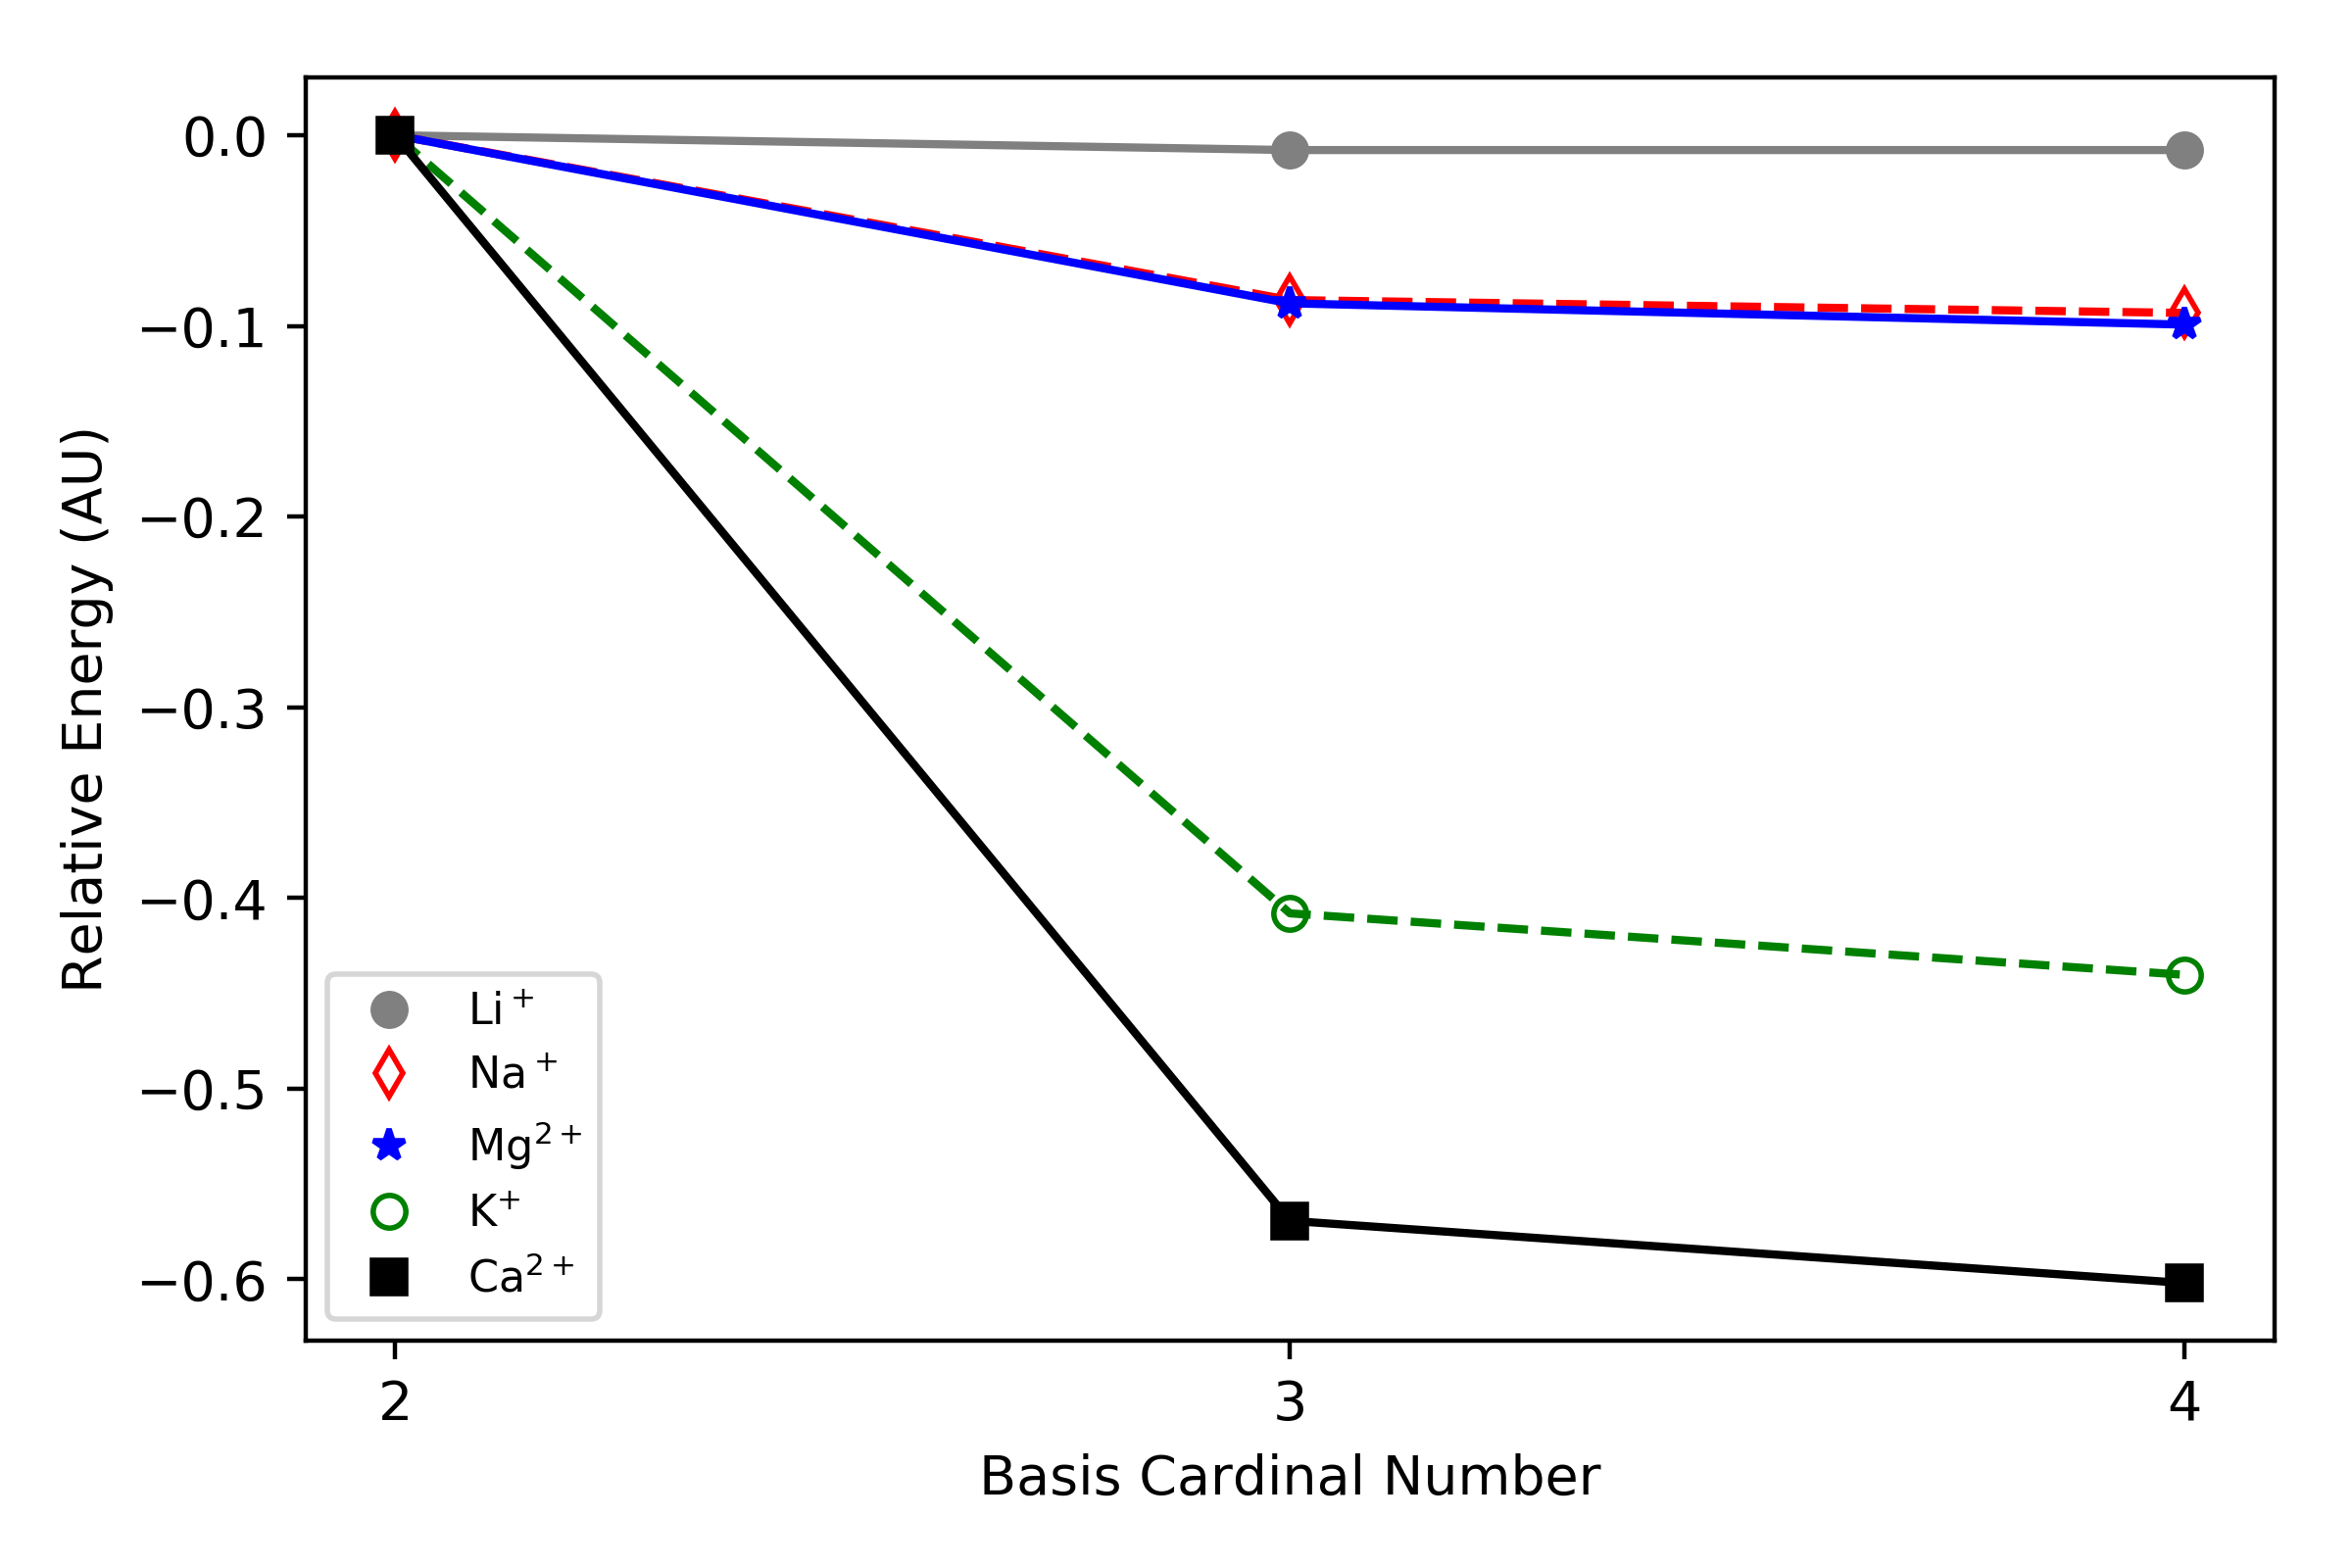
\includegraphics[width=\textwidth]{figures/ap_metals_explicit}
    \caption[Explicitly correlated basis set convergence for alkali and alkaline earth-metal cations.]{Explicitly correlated CCSD(T,Full)-F12$^*$/Def2-$X$ ($X$=SVP,TZVPPD,QZVPPD) basis set convergence for alkali and alkaline earth-metal cations. The relative energy of each basis set relative to the cc-pVCDZ for each metal. The cardinal number of the basis sets is $X$.}
  \label{fig:ap_metals_explicit}
\end{figure}
